\chapter{Simulation Results}

\section{Time to Default Route Detection}
\label{Appx:cdf}
\subsection{Line Scenario}
\label{Appx:cdf:line}
%%%%%%%%%%%%%% line9 %%%%%%%%%%%%%%%%%%%%%%%%%%%%%%%%%%%%%
\begin{figure}[htpb]
  \begin{center}
    \leavevmode
      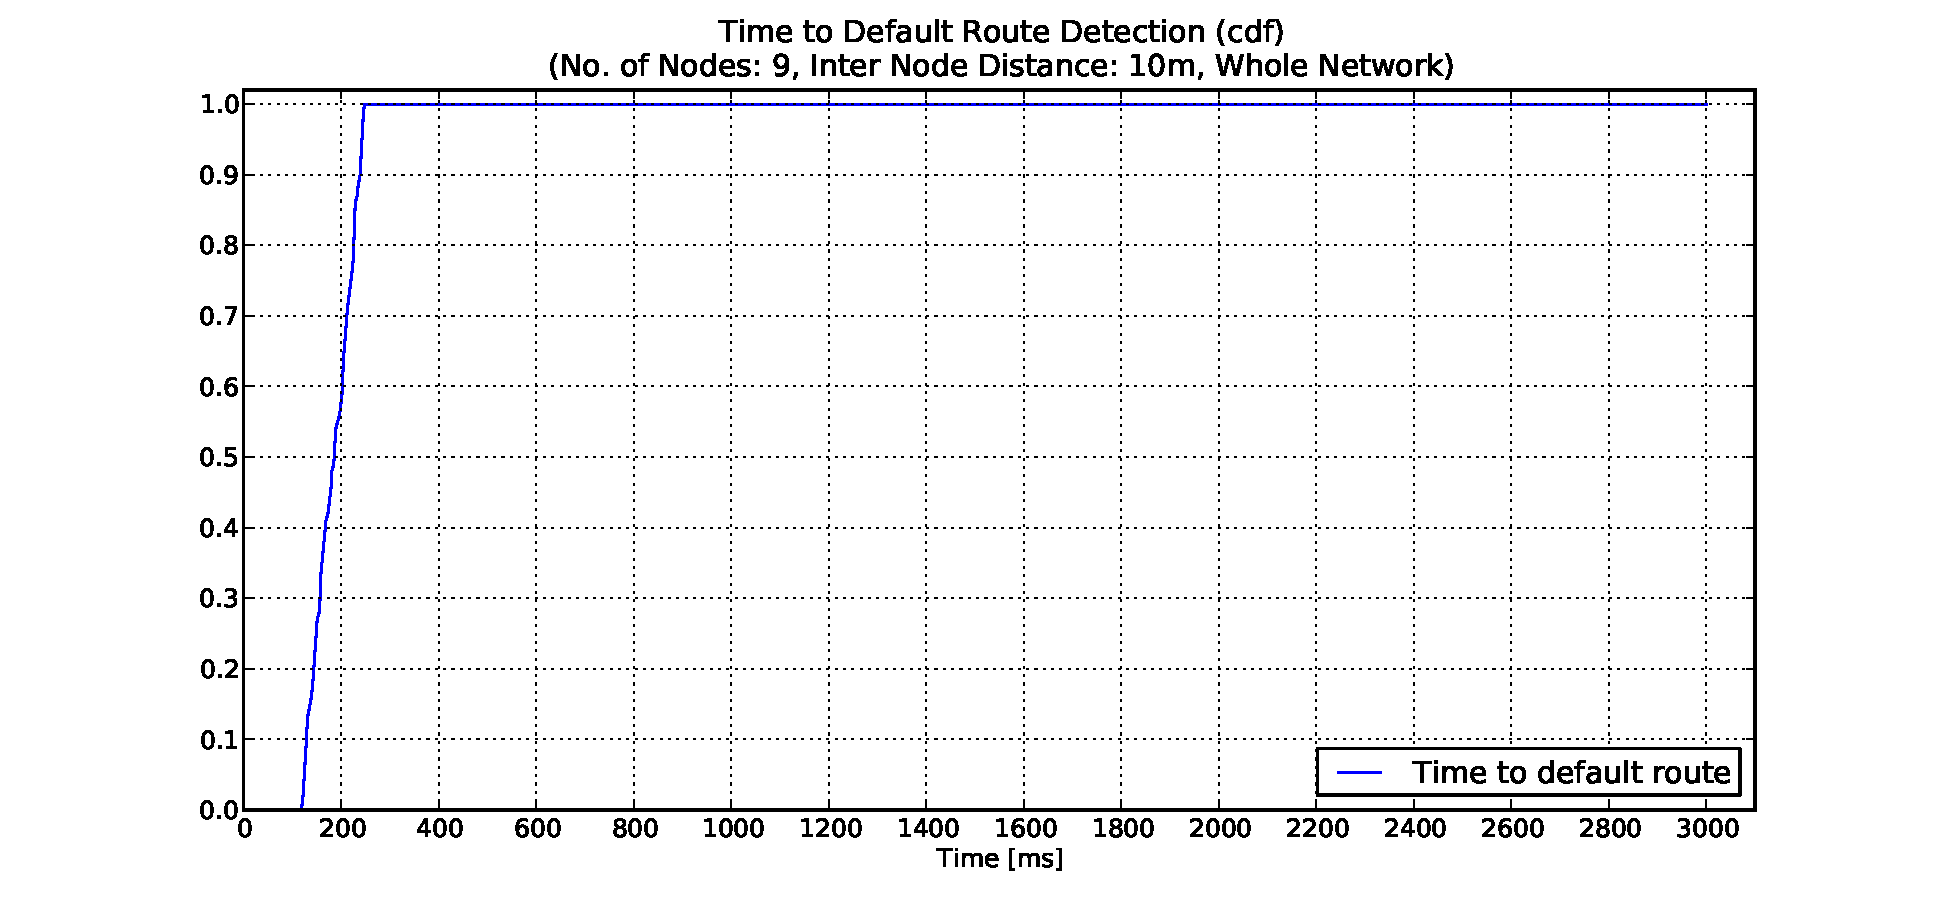
\includegraphics[scale=0.38]
      {Pics/results/9/MRHOF/line/dist10_montecarlo_cdf_hist.pdf}
   \caption{CDF of default route discovery time: 9-node line scenario with 10 m internode distance}
   \label{fig:9_MRHOF_line_10_cdf}
  \end{center}
\end{figure}

\begin{figure}[htpb]
  \begin{center}
    \leavevmode
        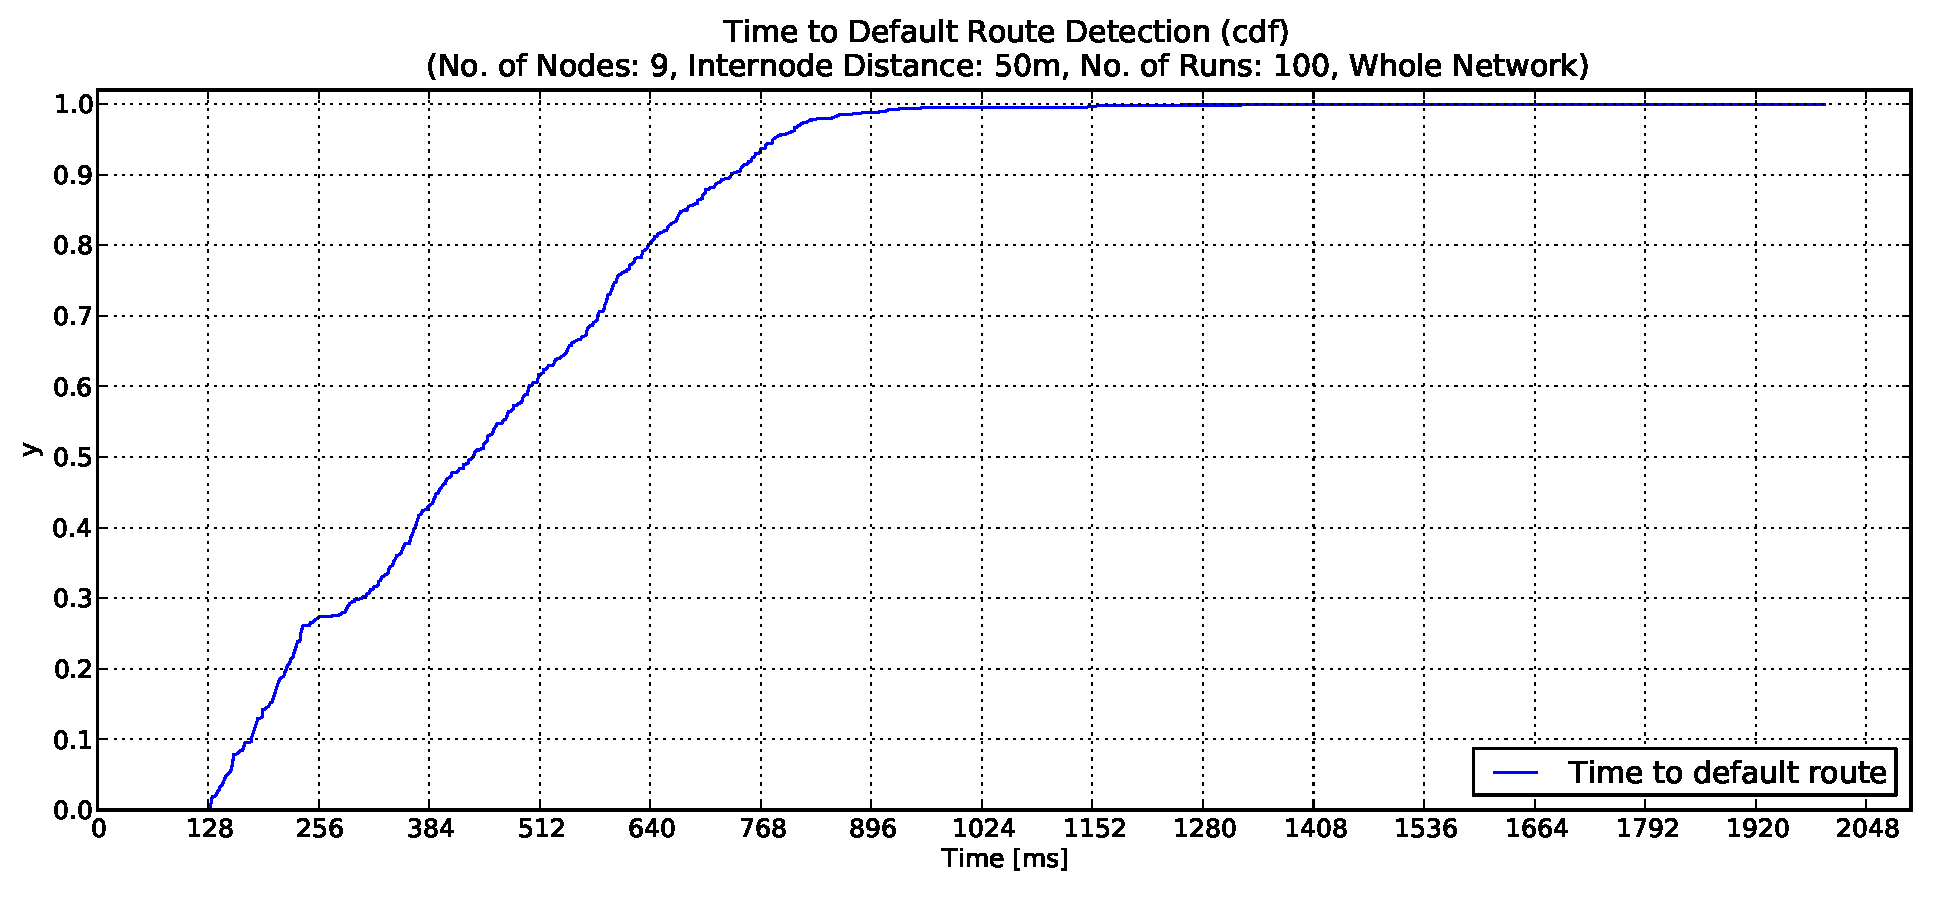
\includegraphics[scale=0.38]
      {Pics/results/9/MRHOF/line/dist50_montecarlo_cdf_hist.pdf}
   \caption{CDF of default route discovery time: 9-node line scenario with 50 m internode distance}
   \label{fig:9_MRHOF_line_50_cdf}
  \end{center}
\end{figure}

\begin{figure}[htpb]
  \begin{center}
    \leavevmode
      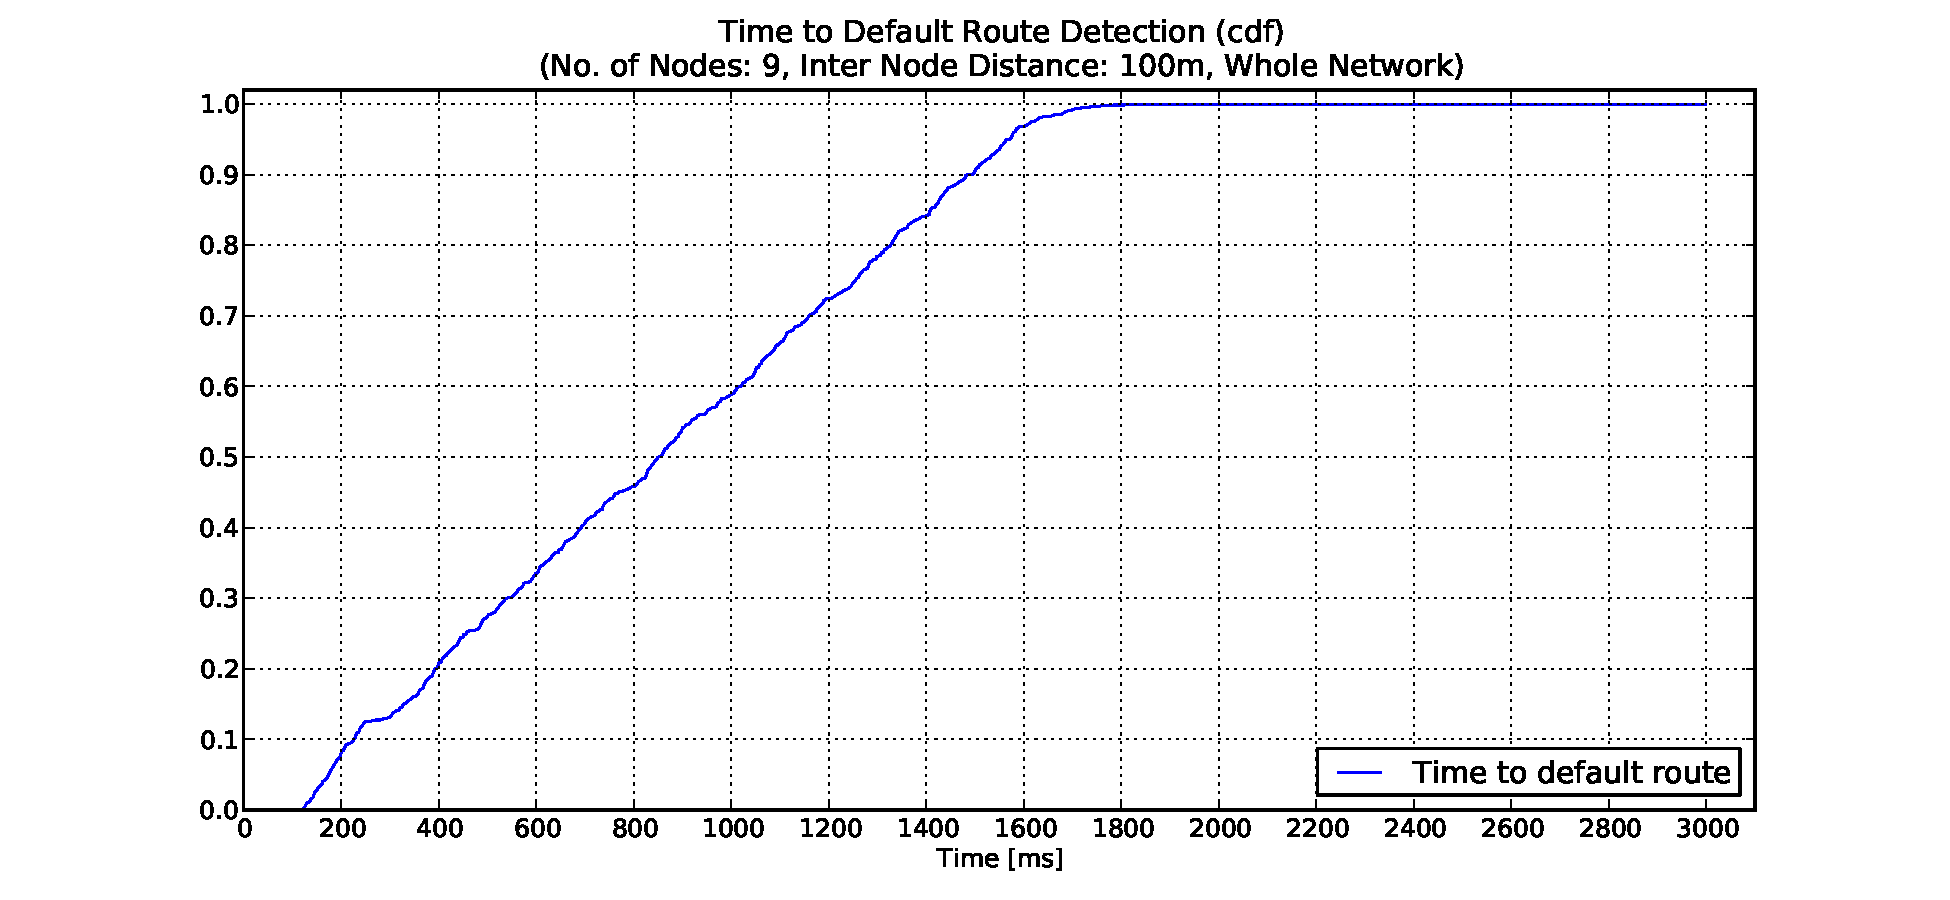
\includegraphics[scale=0.38]
      {Pics/results/9/MRHOF/line/dist100_montecarlo_cdf_hist.pdf}
   \caption{CDF of default route discovery time: 9-node line scenario with 100 m internode distance}
   \label{fig:9_MRHOF_line100_cdf}
  \end{center}
\end{figure}

%%%%%%%%%%%%%% line16 %%%%%%%%%%%%%%%%%%%%%%%%%%%%%%%%%%%%%

\begin{figure}[htpb]
  \begin{center}
    \leavevmode
      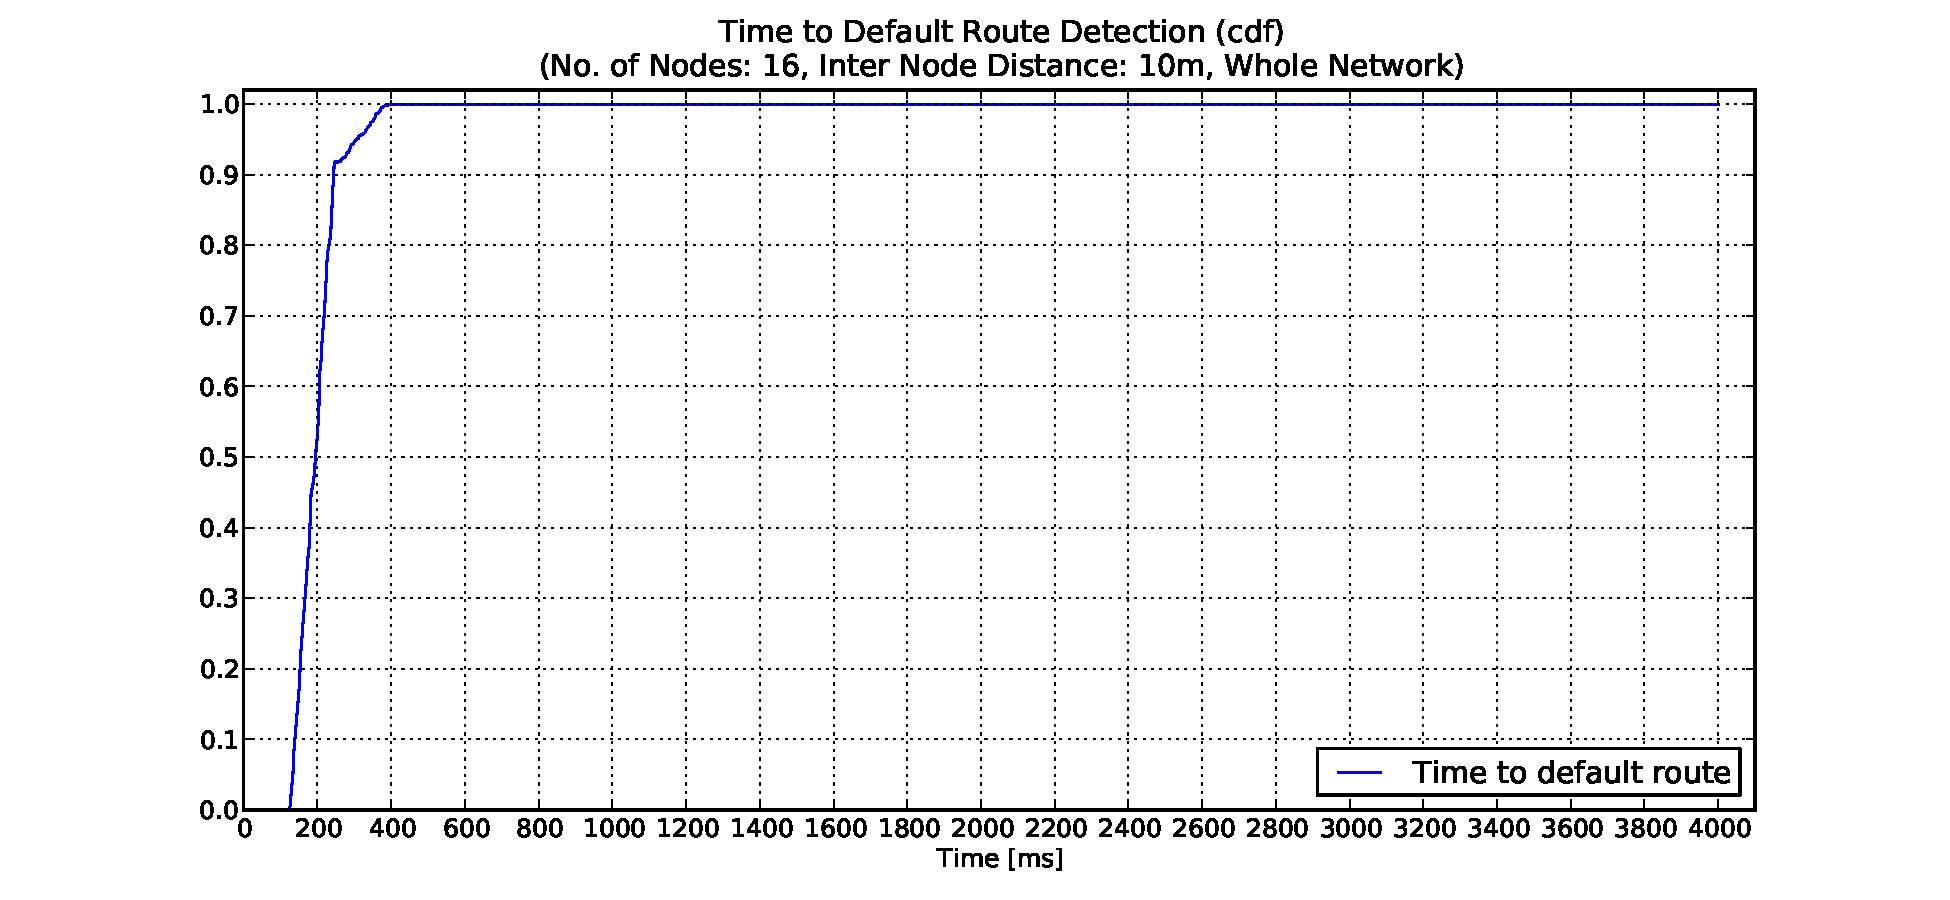
\includegraphics[scale=0.38]
      {Pics/results/16/MRHOF/line/dist10_montecarlo_cdf_hist.pdf}
   \caption{CDF of default route discovery time: 16-node line scenario with 10 m internode distance}
   \label{fig:16_MRHOF_line_10_cdf}
  \end{center}
\end{figure}

\begin{figure}[htpb]
  \begin{center}
    \leavevmode
      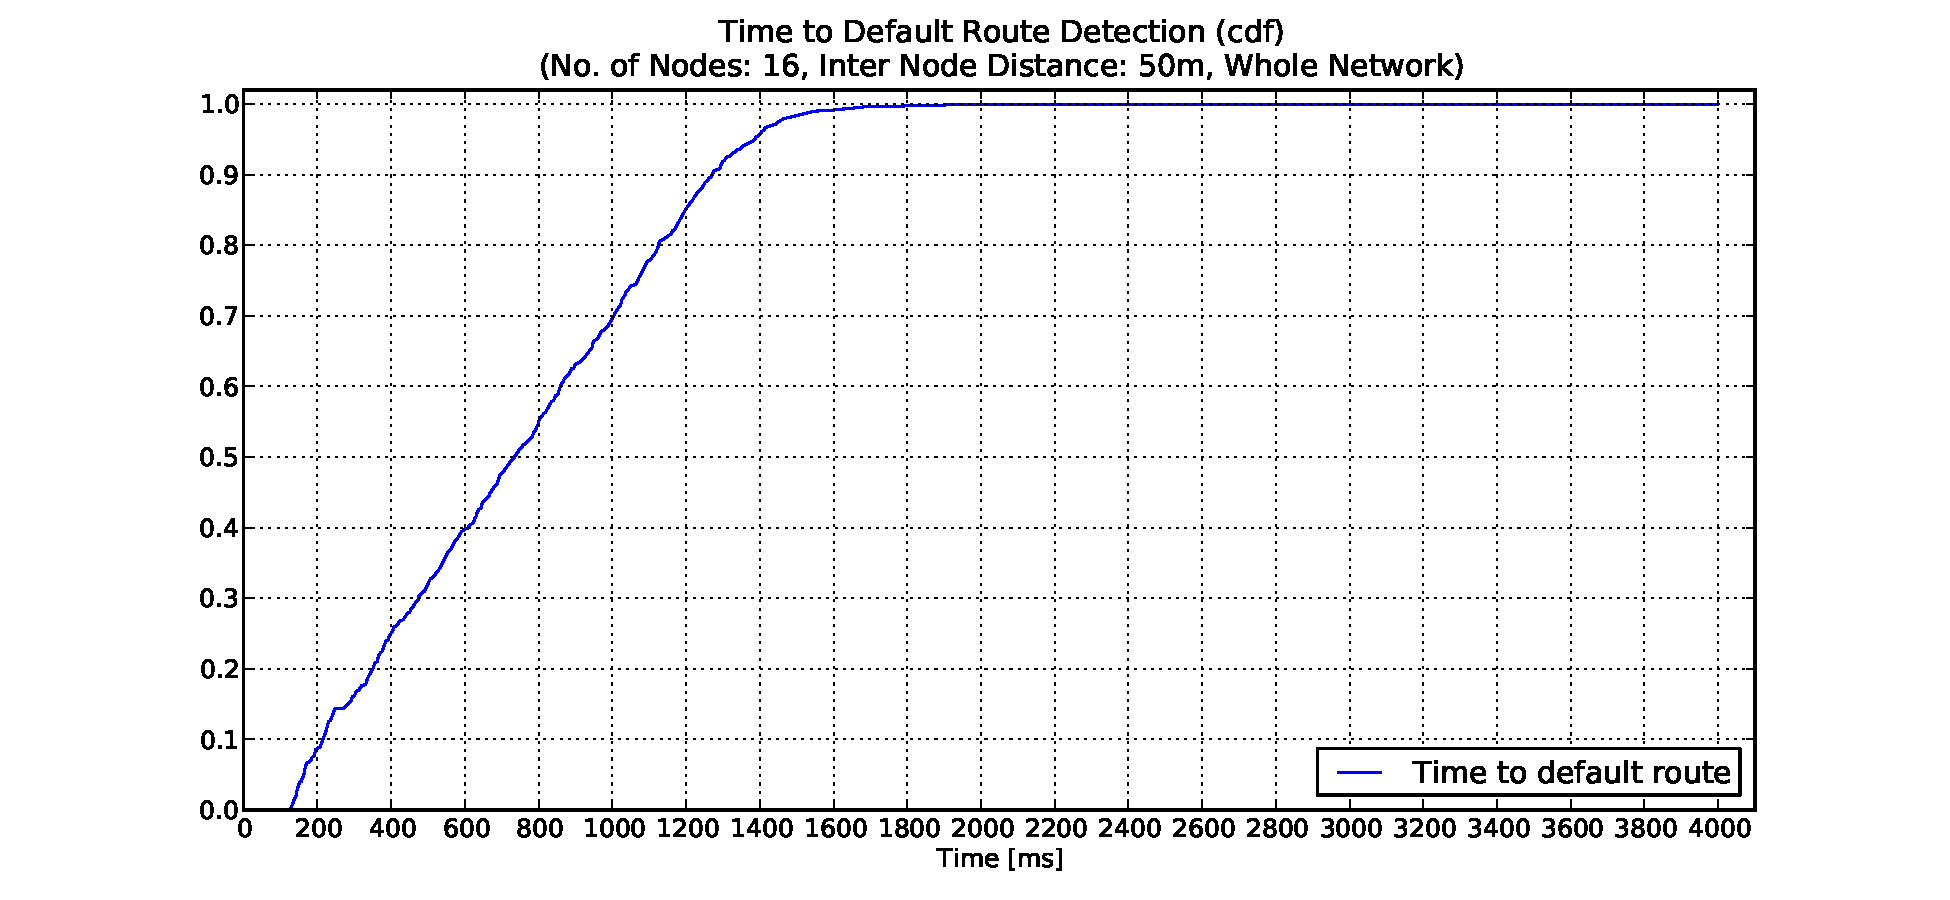
\includegraphics[scale=0.38]
      {Pics/results/16/MRHOF/line/dist50_montecarlo_cdf_hist.pdf}
   \caption{CDF of default route discovery time: 16-node line scenario with 50 m internode distance}
   \label{fig:16_MRHOF_line_50_cdf}
  \end{center}
\end{figure}

\begin{figure}[htpb]
  \begin{center}
  %\vspace{-50pt}
    \leavevmode
      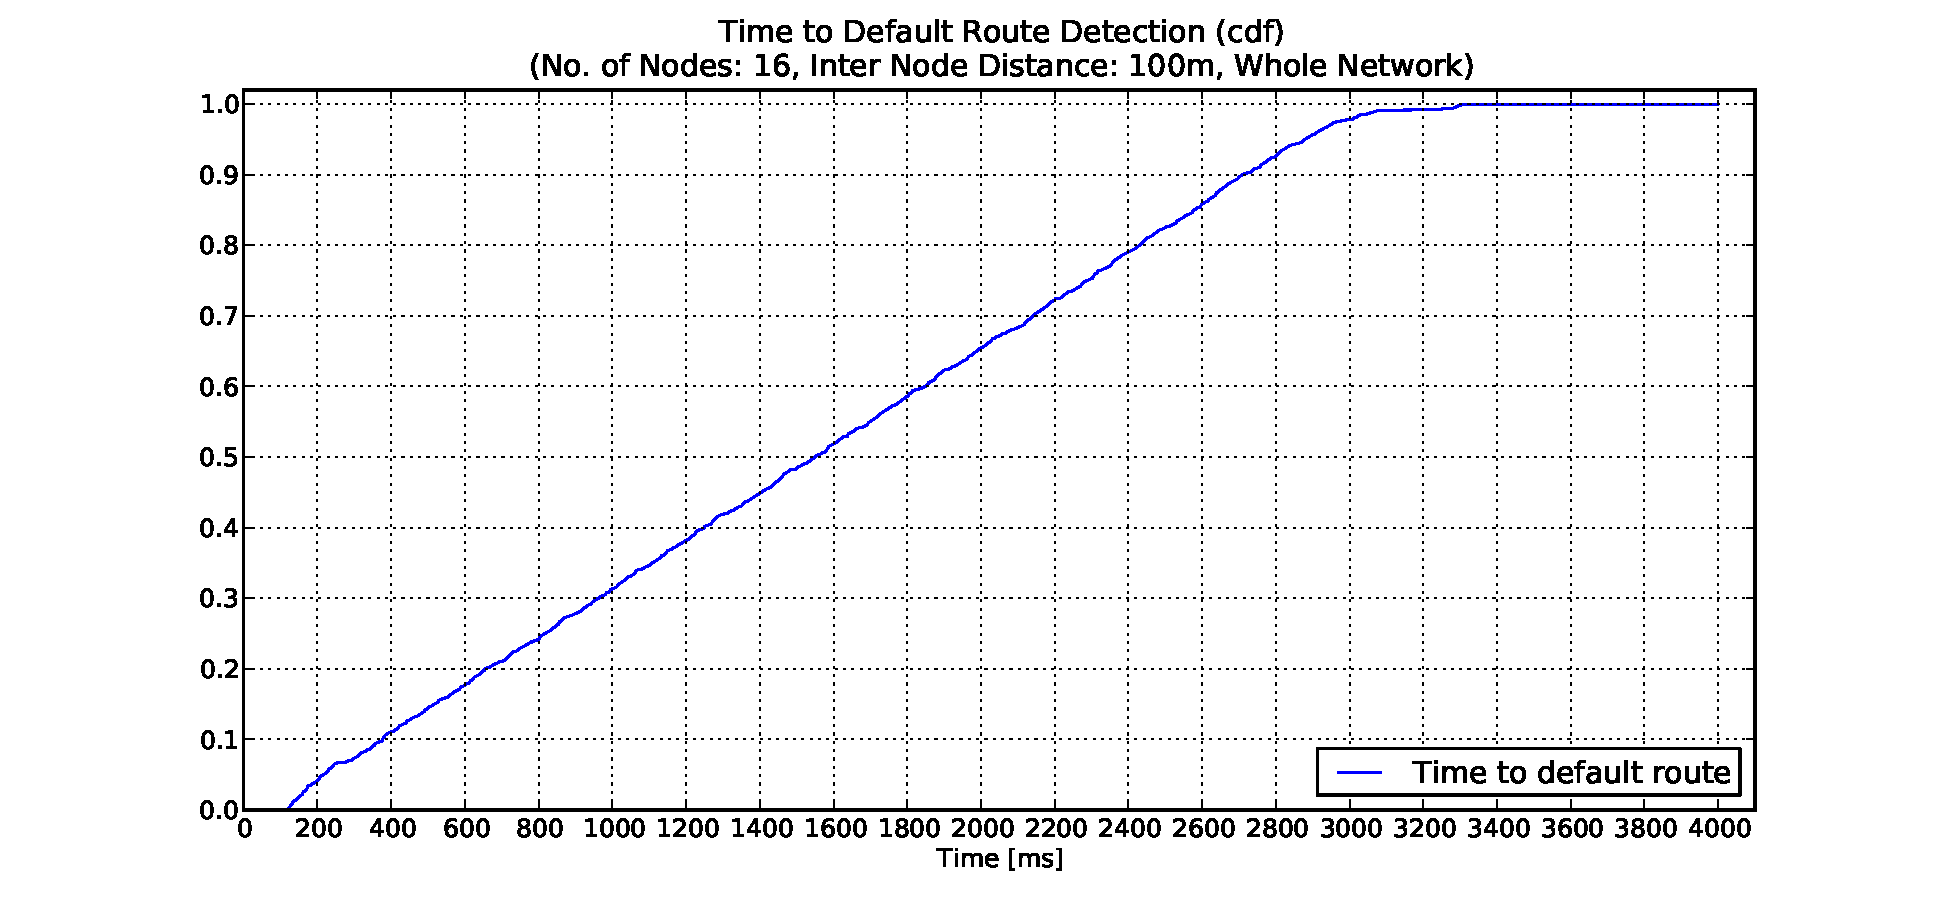
\includegraphics[scale=0.38]
      {Pics/results/16/MRHOF/line/dist100_montecarlo_cdf_hist.pdf}
   \caption{CDF of default route discovery time: 16-node line scenario with 100 m internode distance}
   \label{fig:16_MRHOF_line_100_cdf}
    \vspace{6in}
  \end{center}
\end{figure}

%%%%%%%%%%%%%%%%%%%%%%%%%%%%%%%%%%%%%%%%%%%%%%%%%%%%%%
\clearpage
\subsection{Grid Scenario}
\label{Appx:cdf:grid}

%%%%%%%%%%%%%% grid4 %%%%%%%%%%%%%%%%%%%%%%%%%%%%%%%%%%%%%
\begin{figure}[h]
  \begin{center}
  \vspace{-10pt}
    \leavevmode
      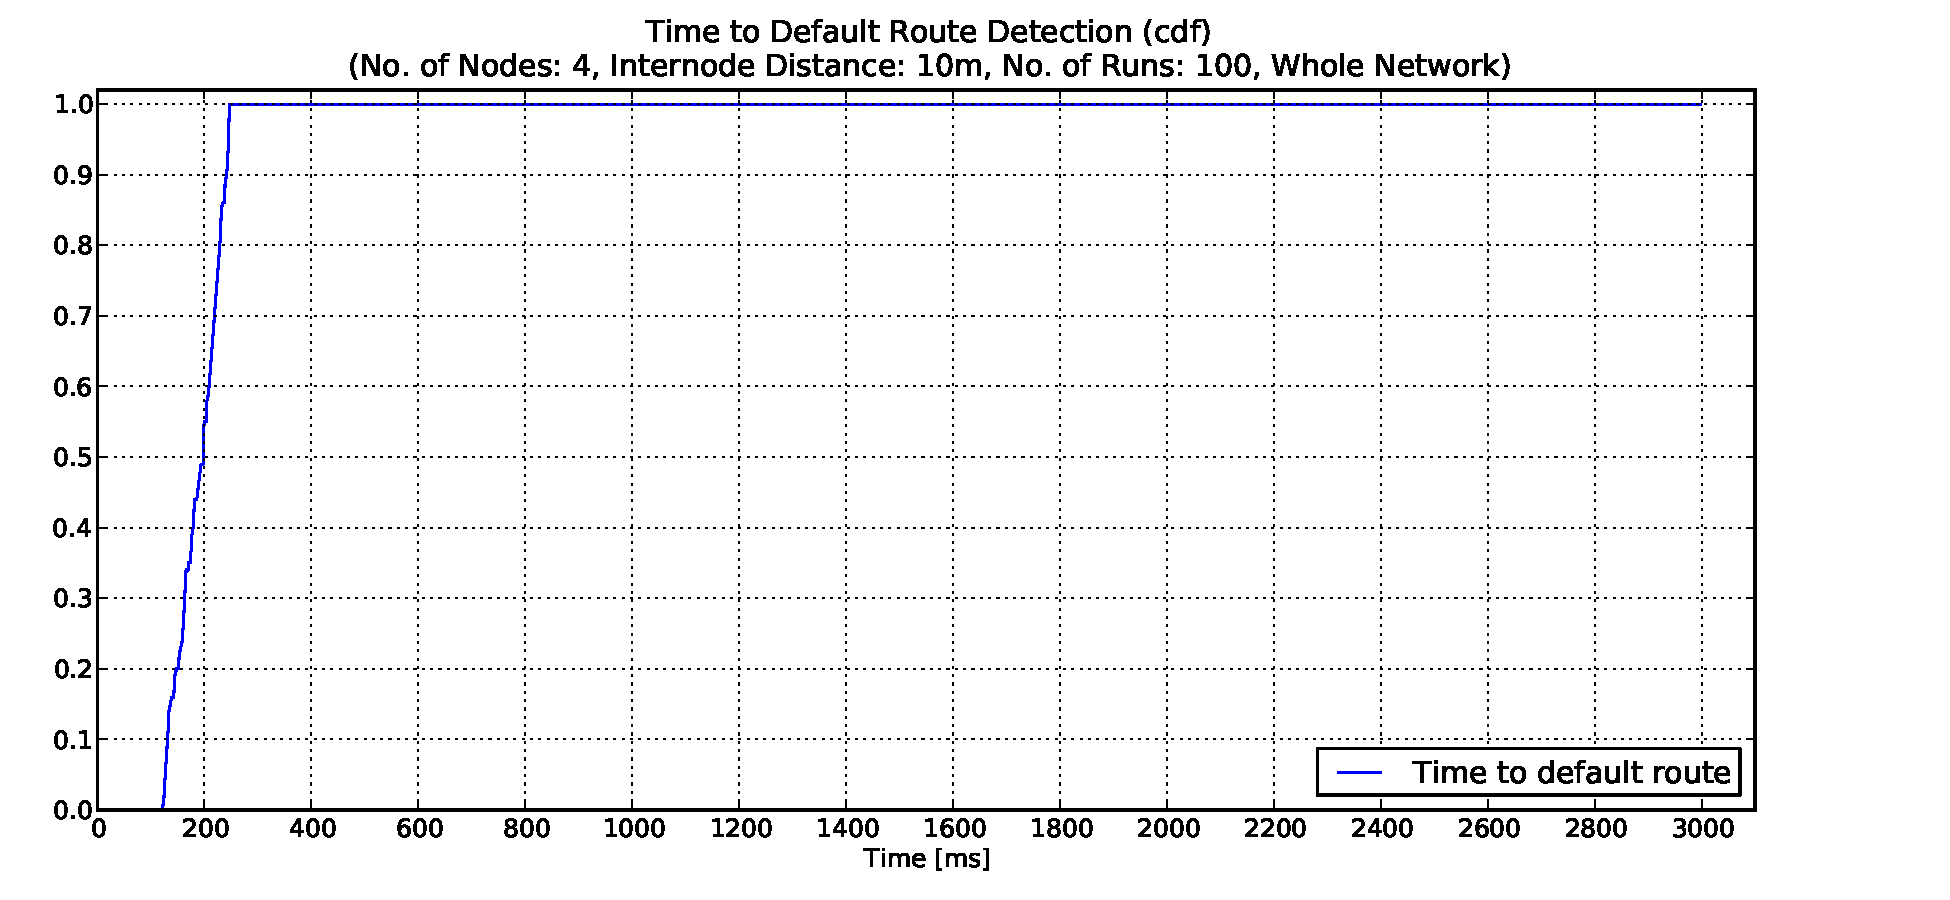
\includegraphics[scale=0.38]
      {Pics/results/4/MRHOF/grid/dist10_montecarlo_cdf_hist.pdf}
   \caption{CDF of default route discovery time: 4-node grid scenario with 10 m internode distance}
   \label{fig:4_MRHOF_grid_10_cdf}
  \end{center}
\end{figure}

\begin{figure}[htpb]
  \begin{center}
  \vspace{-20pt}
    \leavevmode
      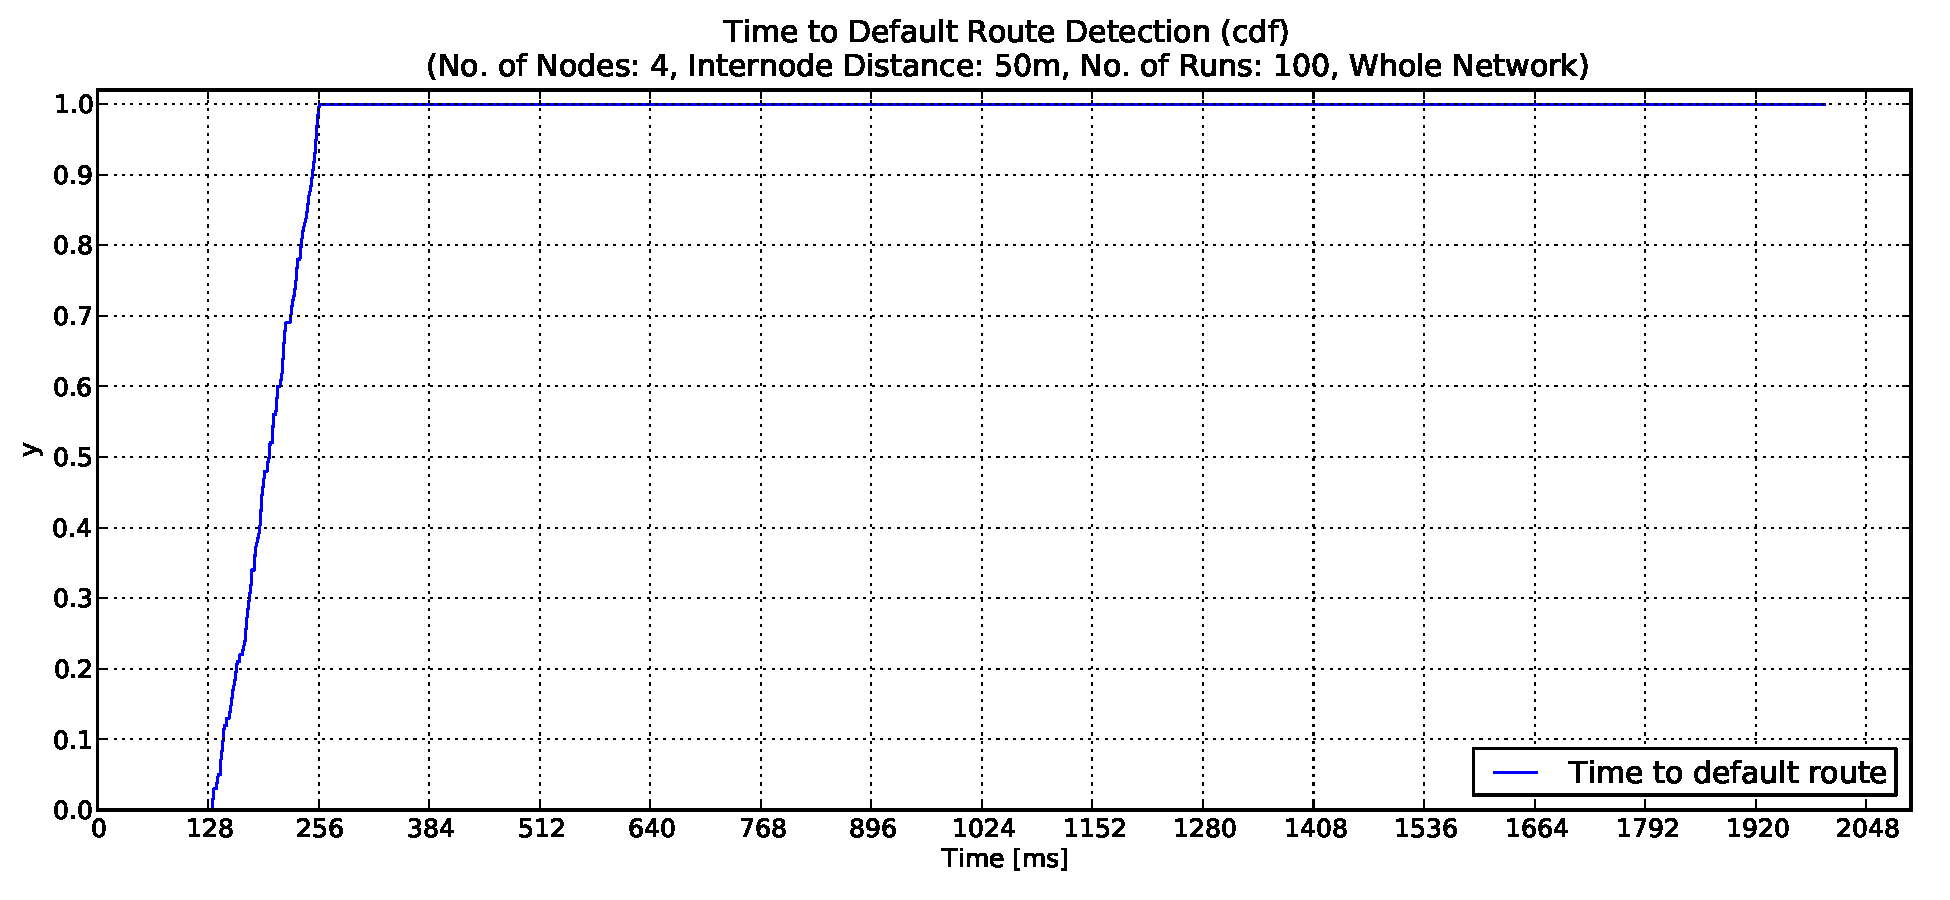
\includegraphics[scale=0.38]
      {Pics/results/4/MRHOF/grid/dist50_montecarlo_cdf_hist.pdf}
   \caption{CDF of default route discovery time: 4-node grid scenario with 50 m internode distance}
   \label{fig:4_MRHOF_grid_50_cdf}
  \end{center}
\end{figure}

\begin{figure}[htb]
  \begin{center}
  \vspace{-20pt}
    \leavevmode
      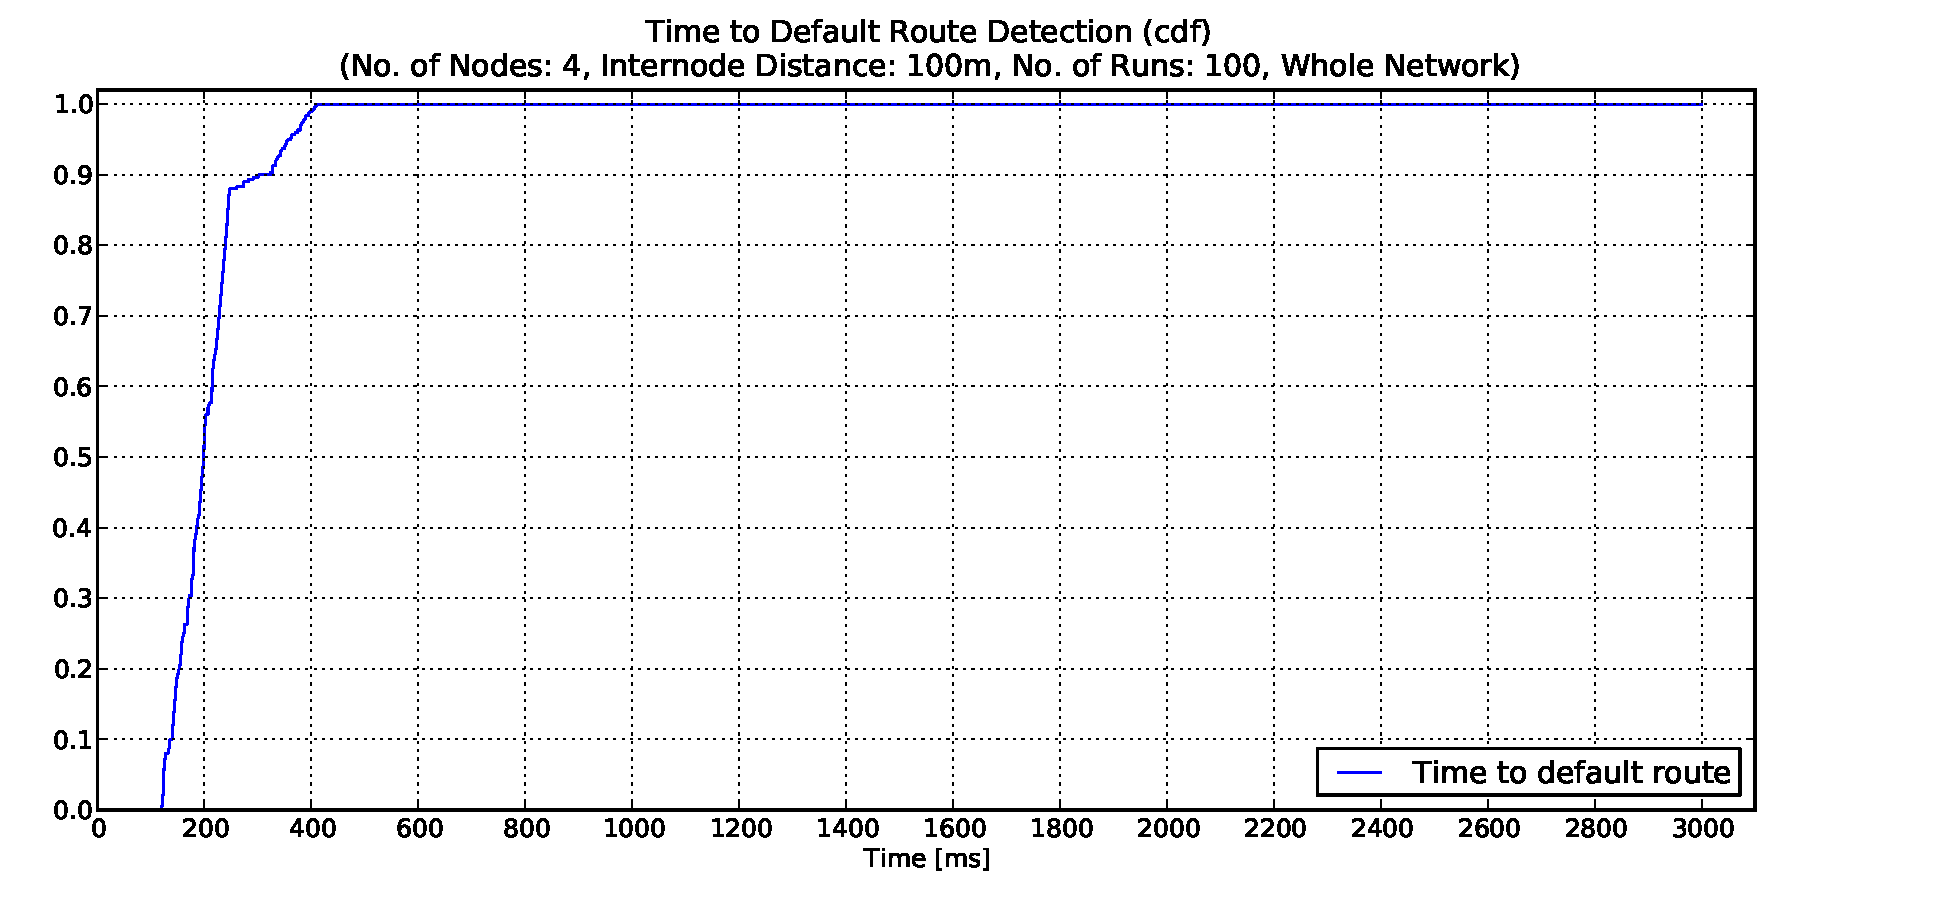
\includegraphics[scale=0.38]
      {Pics/results/4/MRHOF/grid/dist100_montecarlo_cdf_hist.pdf}
   \caption{CDF of default route discovery time: 4-node grid scenario with 100 m internode distance}
   \label{fig:4_MRHOF_grid_100_cdf}
  \end{center}
\end{figure}

%%%%%%%%%%%%%% grid9 %%%%%%%%%%%%%%%%%%%%%%%%%%%%%%%%%%%%%
\begin{figure}[htpb]
  \begin{center}
   \vspace{-20pt}
    \leavevmode
      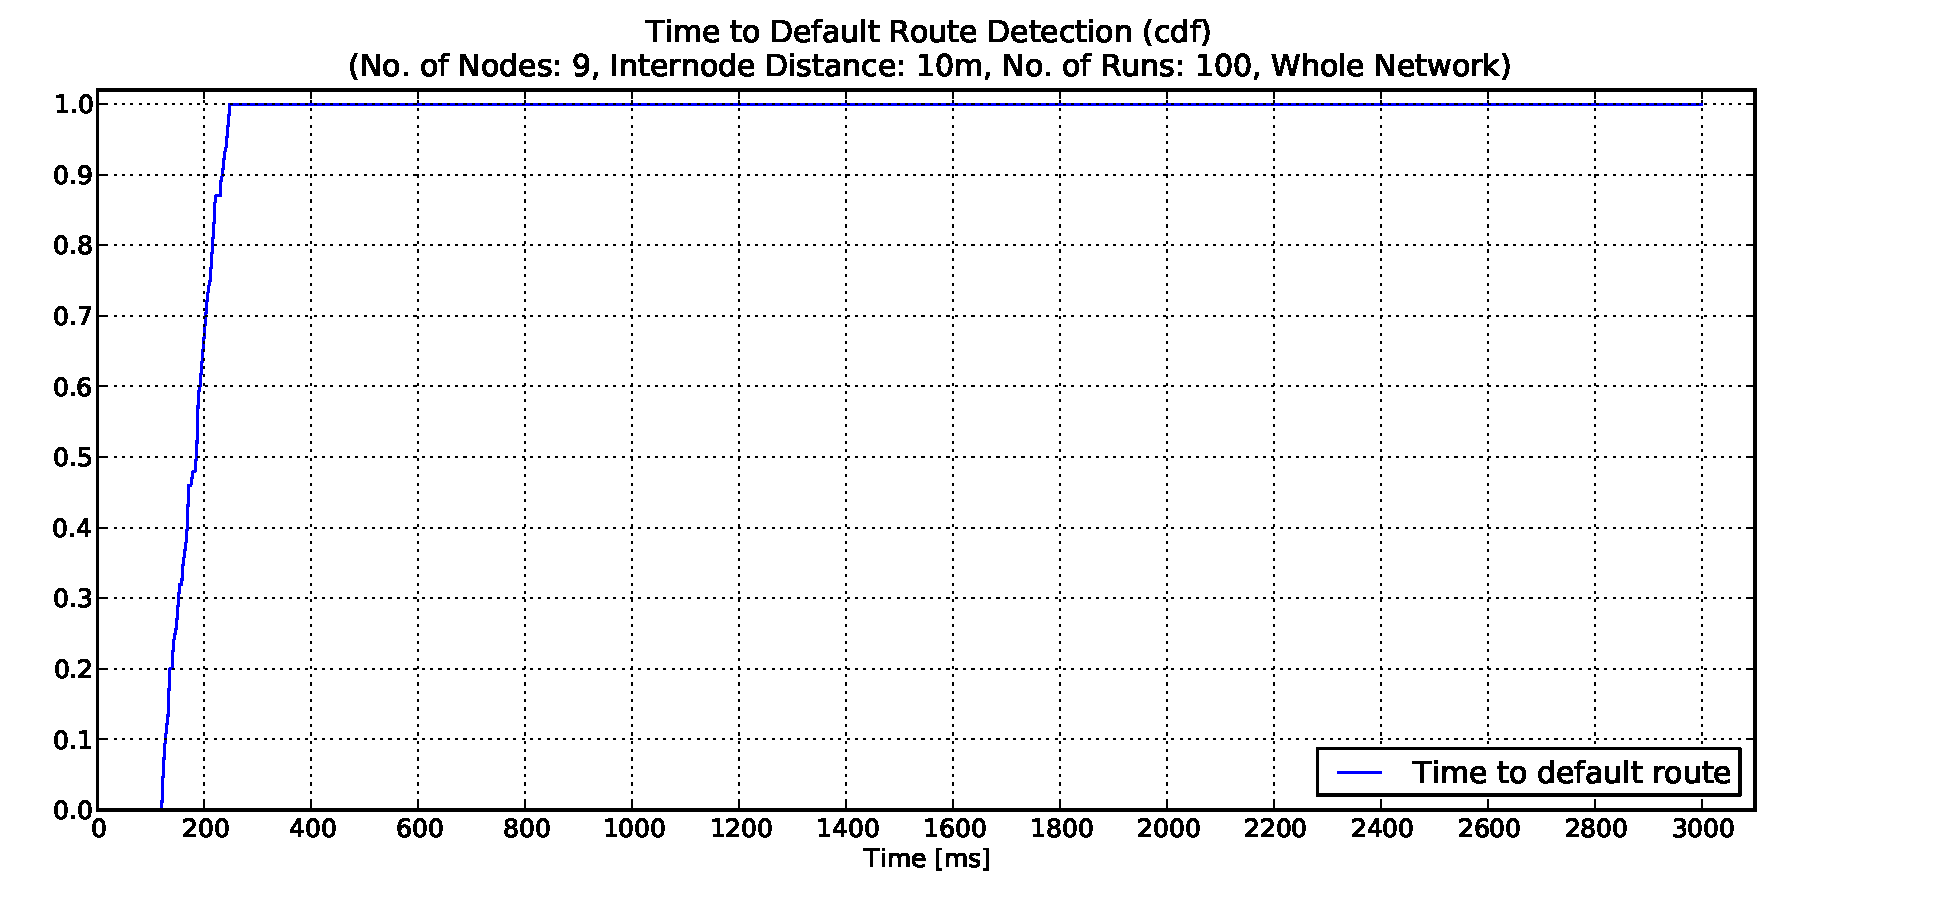
\includegraphics[scale=0.38]
      {Pics/results/9/MRHOF/grid/dist10_montecarlo_cdf_hist.pdf}
   \caption{CDF of default route discovery time: 9-node grid scenario with 10 m internode distance}
   \label{fig:9_MRHOF_grid_10_cdf}
  \end{center}
\end{figure}

\begin{figure}[htpb]
  \begin{center}
   \vspace{-20pt}
    \leavevmode
      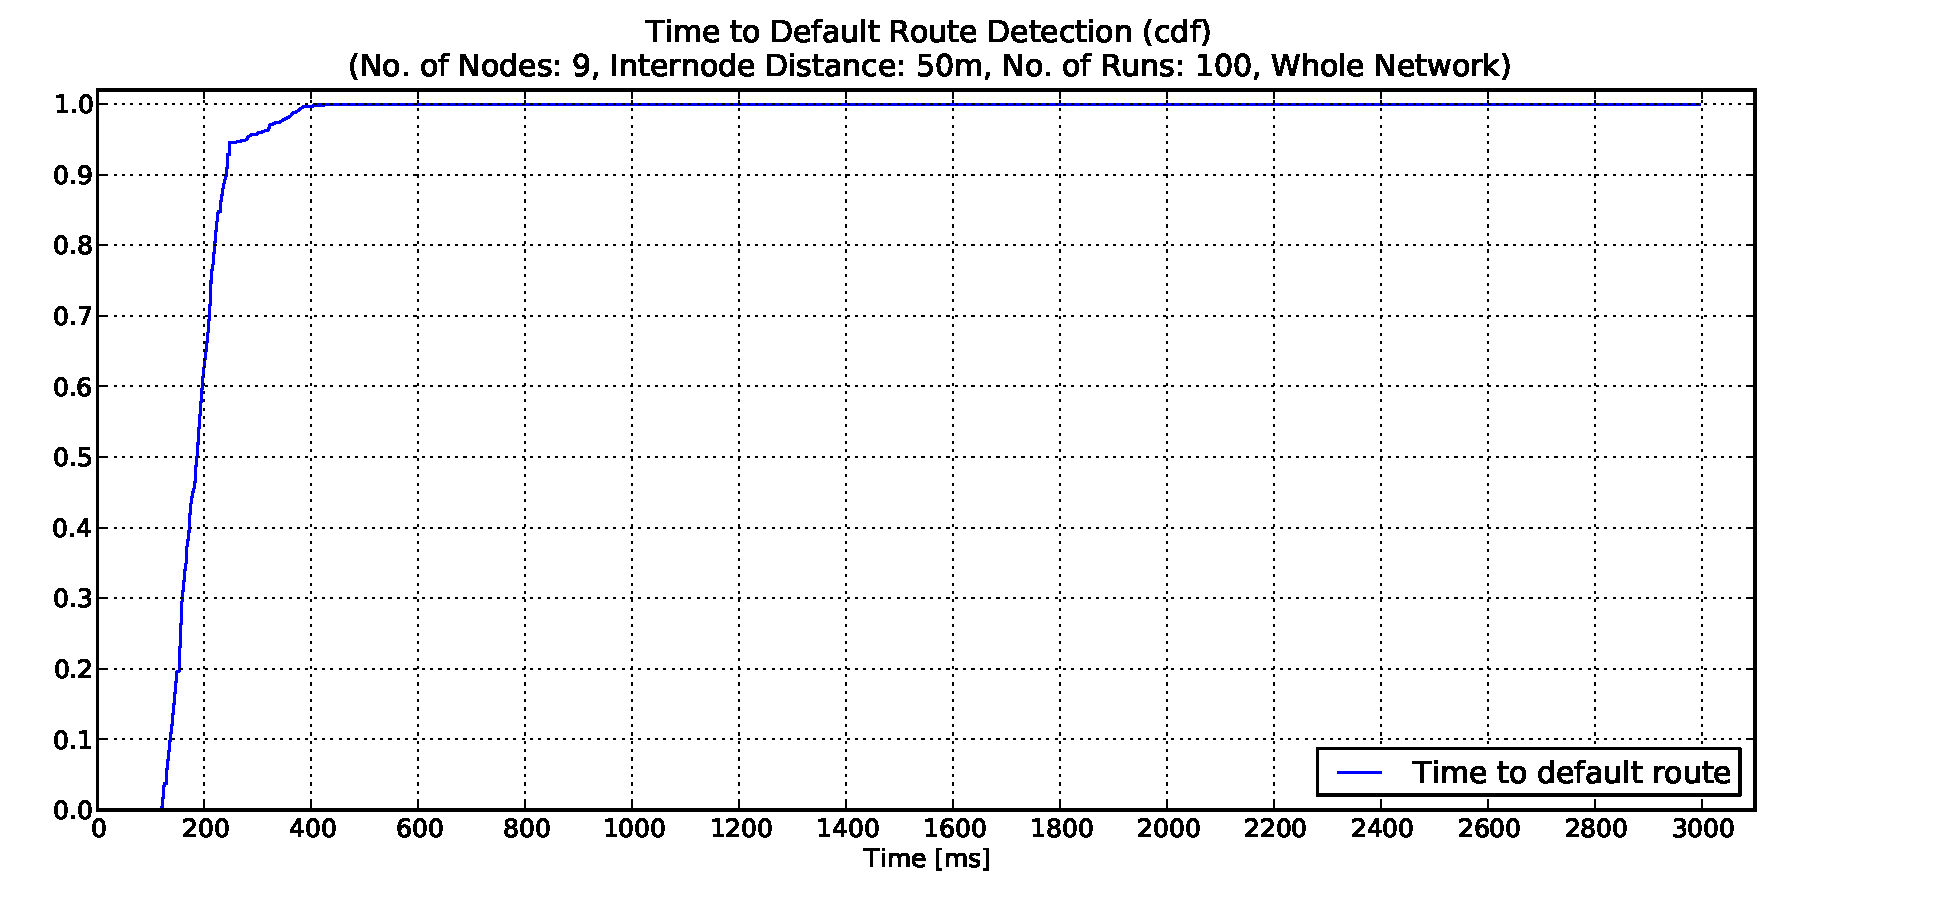
\includegraphics[scale=0.38]
      {Pics/results/9/MRHOF/grid/dist50_montecarlo_cdf_hist.pdf}
   \caption{CDF of default route discovery time: 9-node grid scenario with 50 m internode distance}
   \label{fig:9_MRHOF_grid_50_cdf}
  \end{center}
\end{figure}

\begin{figure}[htpb]
  \begin{center}
   \vspace{-20pt}
    \leavevmode
      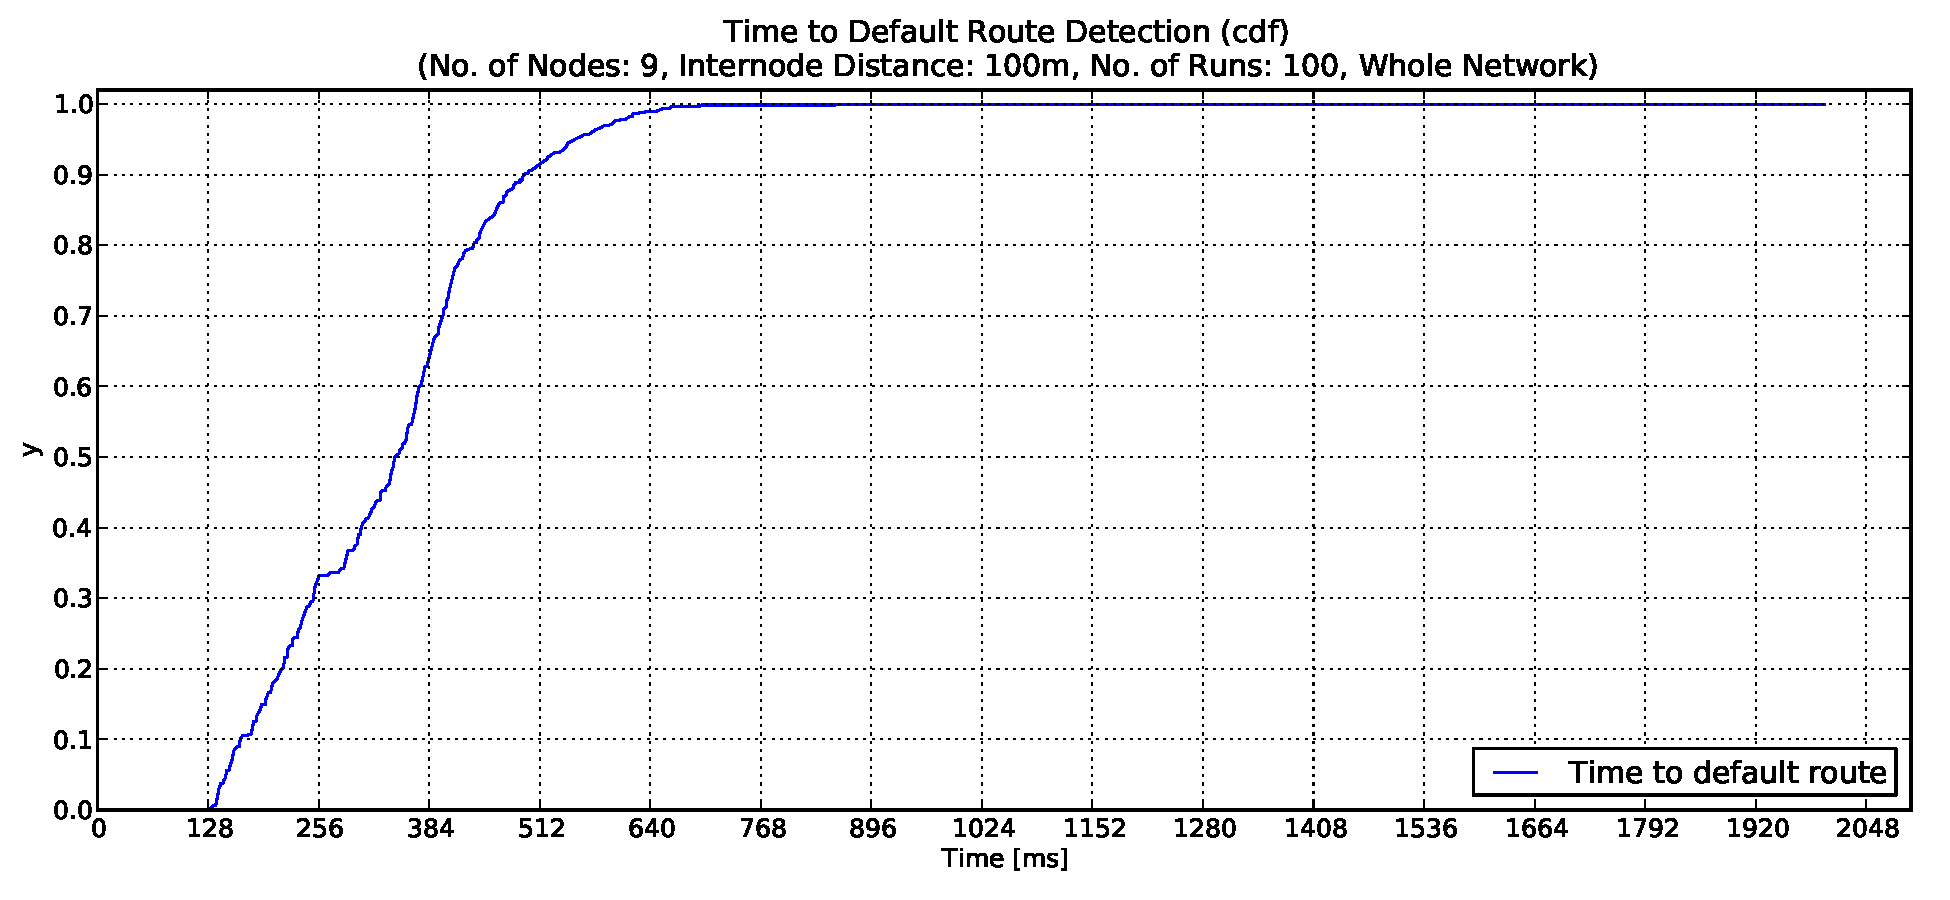
\includegraphics[scale=0.38]
      {Pics/results/9/MRHOF/grid/dist100_montecarlo_cdf_hist.pdf}
   \caption{CDF of default route discovery time: 9-node grid scenario with 100 m internode distance}
   \label{fig:9_MRHOF_grid_100_cdf}
  \end{center}
\end{figure}

%%%%%%%%%%%%%% grid16 %%%%%%%%%%%%%%%%%%%%%%%%%%%%%%%%%%%%%

\begin{figure}[htpb]
  \begin{center}
   \vspace{-20pt}
    \leavevmode
      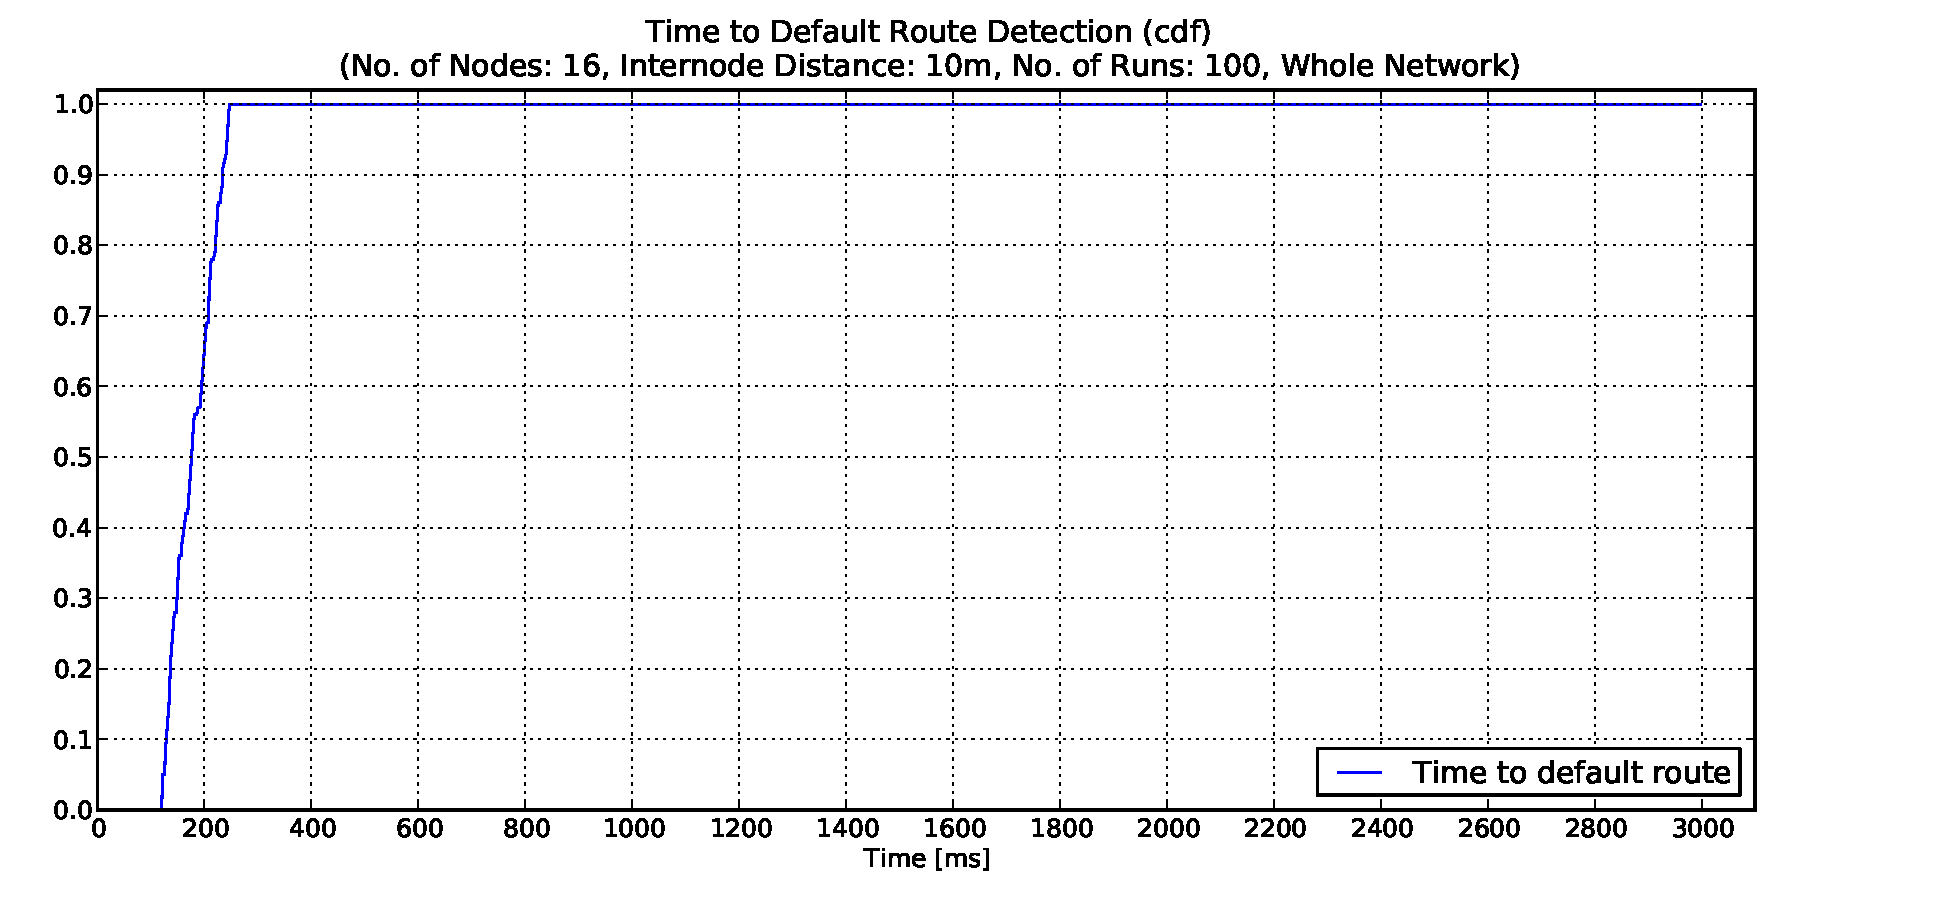
\includegraphics[scale=0.38]
      {Pics/results/16/MRHOF/grid/dist10_montecarlo_cdf_hist.pdf}
   \caption{CDF of default route discovery time: 16-node grid scenario with 10 m internode distance}
   \label{fig:16_MRHOF_grid_10_cdf}
  \end{center}
\end{figure}

\begin{figure}[htpb]
  \begin{center}
   \vspace{-20pt}
    \leavevmode
      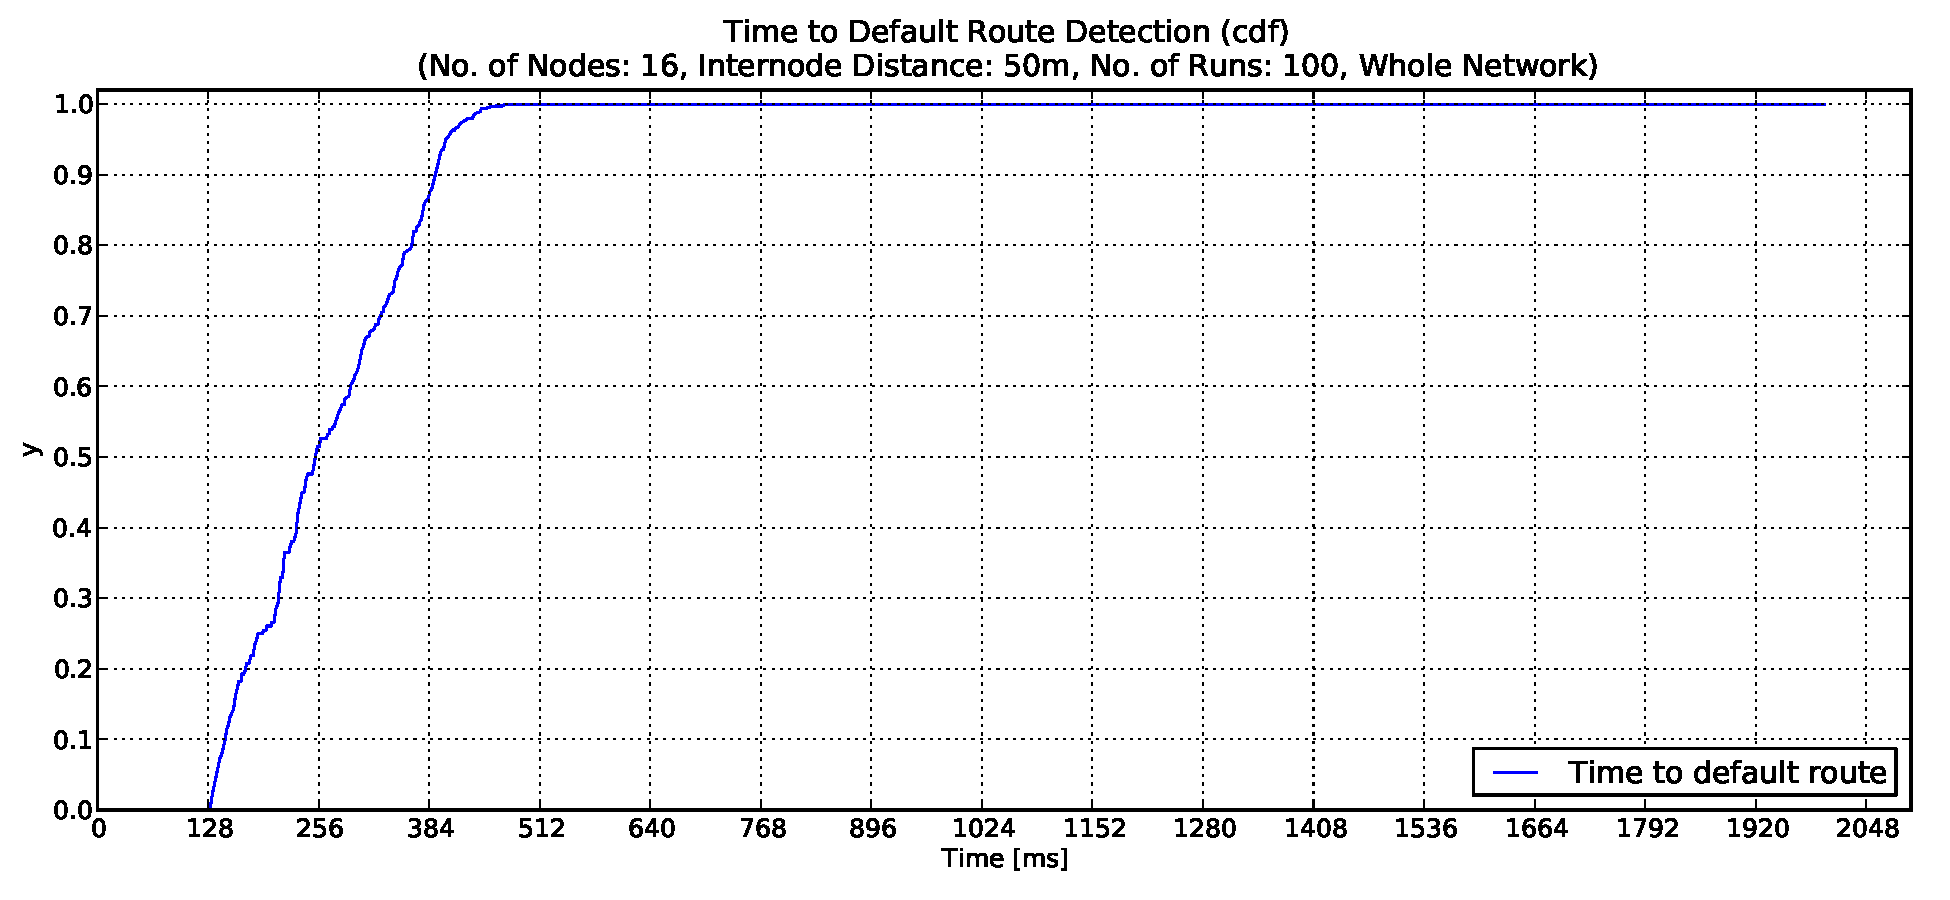
\includegraphics[scale=0.38]
      {Pics/results/16/MRHOF/grid/dist50_montecarlo_cdf_hist.pdf}
   \caption{CDF of default route discovery time: 16-node grid scenario with 50 m internode distance}
   \label{fig:16_MRHOF_grid_50_cdf}
  \end{center}
\end{figure}

\begin{figure}[htpb]
  \begin{center}
   \vspace{-20pt}
    \leavevmode
      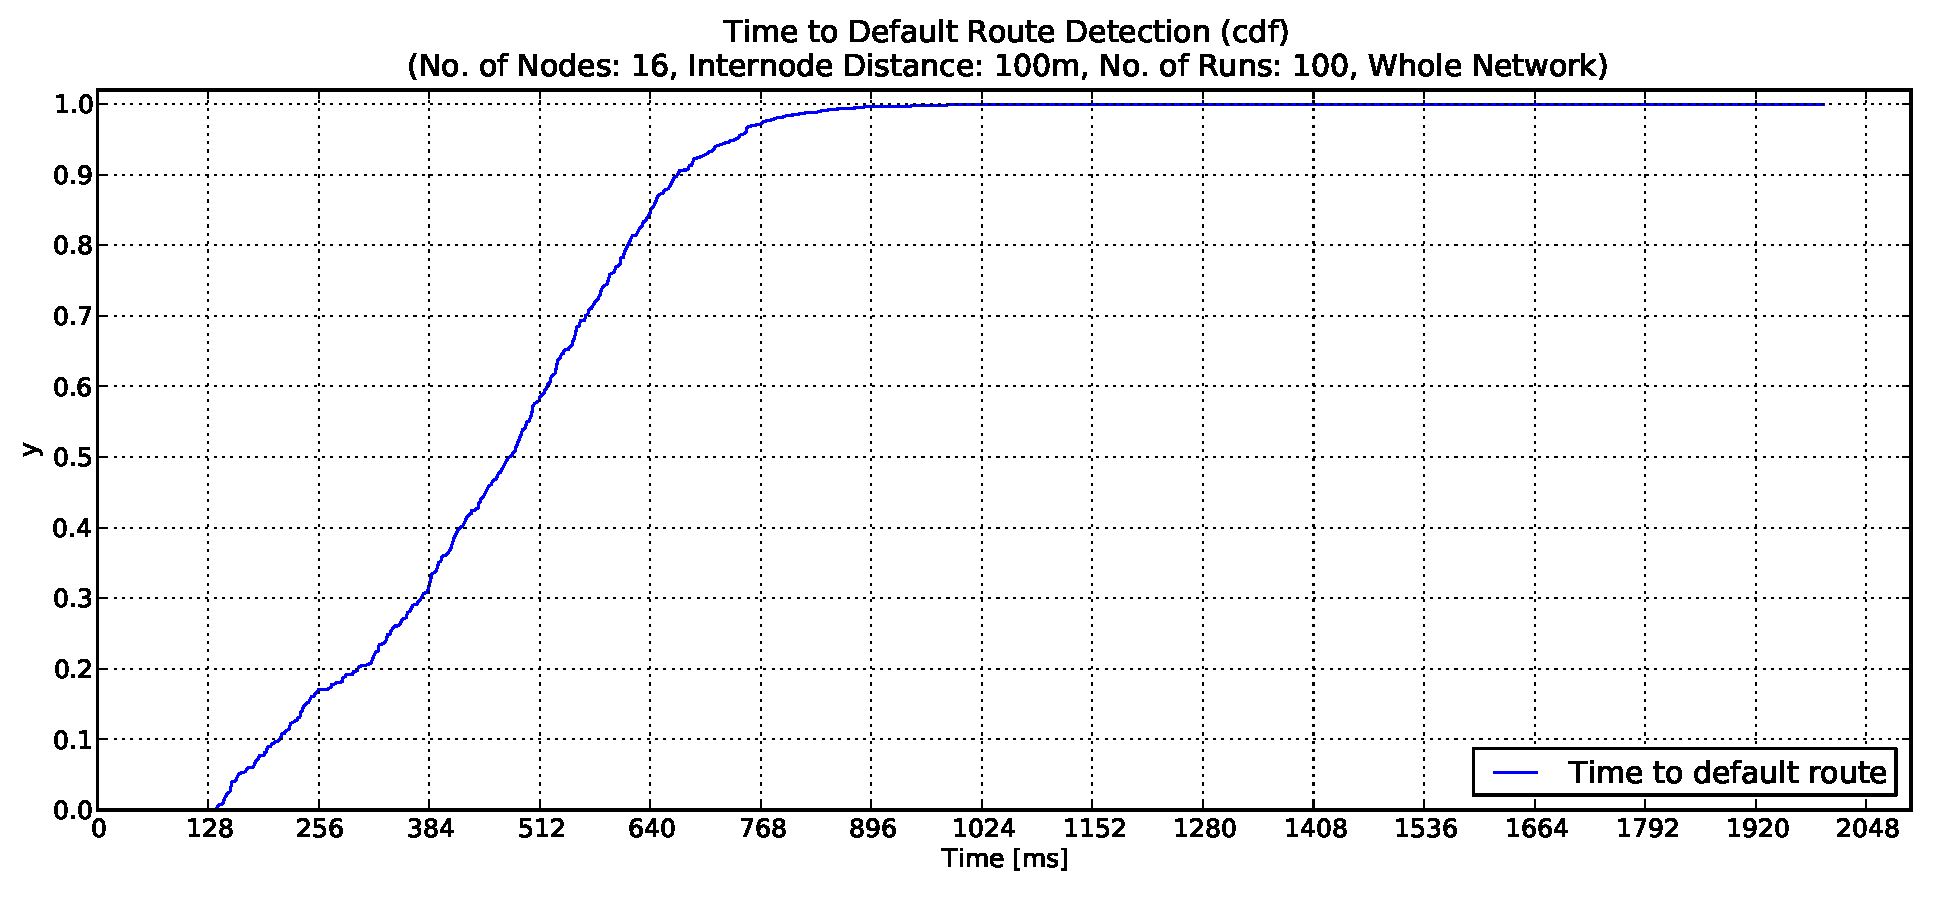
\includegraphics[scale=0.38]
      {Pics/results/16/MRHOF/grid/dist100_montecarlo_cdf_hist.pdf}
   \caption{CDF of default route discovery time: 16-node grid scenario with 100 m internode distance}
   \end{center}
\end{figure}

%%%%%%%%%%%%%%%%%%%%%%%%%%%%%%%%%%% ICMP %%%%%%%%%%%%%%%%%%%%%%%%%%%%%%%%%%%%%%%%
\clearpage
\section{Control Message Overhead}
\label{Appx:icmp}

\subsection{Line Scenario}
\label{Appx:icmp:line}
%%%%%%%%%%%%%%%%%%%%%%%%%%%%%%%%%%% line 16
\begin{figure}[htpb]
  \begin{center}
    \vspace{-10pt}
    \leavevmode
    \subfloat[First 10 minutes]{\label{fig:16_MRHOF_line_10_icmp0}
      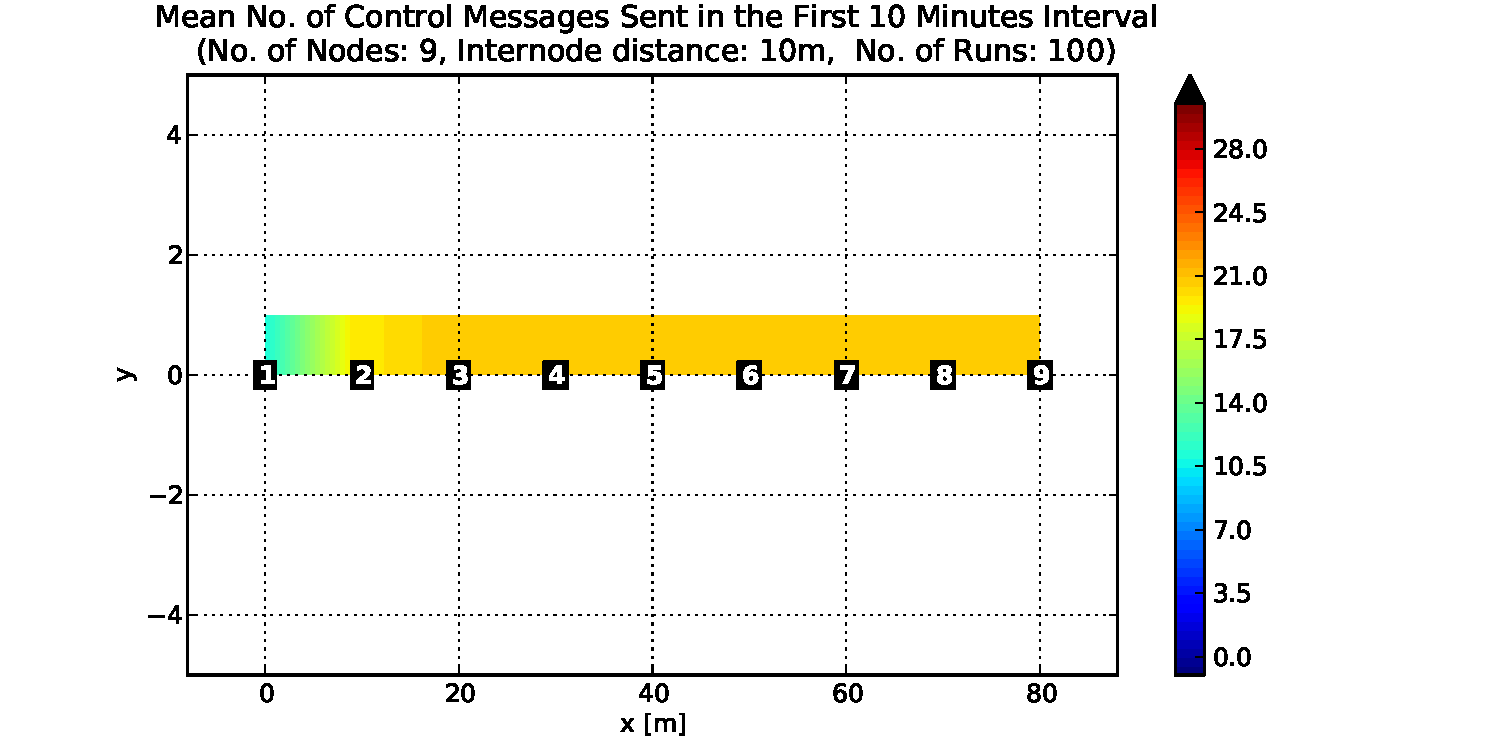
\includegraphics[trim=1.7cm 0cm 3cm 0cm, clip=true, scale=0.38]{Pics/results/9/MRHOF/line/dist10_montecarlo_contour_sent_ICMP_0.pdf}}
    \subfloat[Second 10 minutes]{\label{fig:16_MRHOF_line_10_icmp1}
       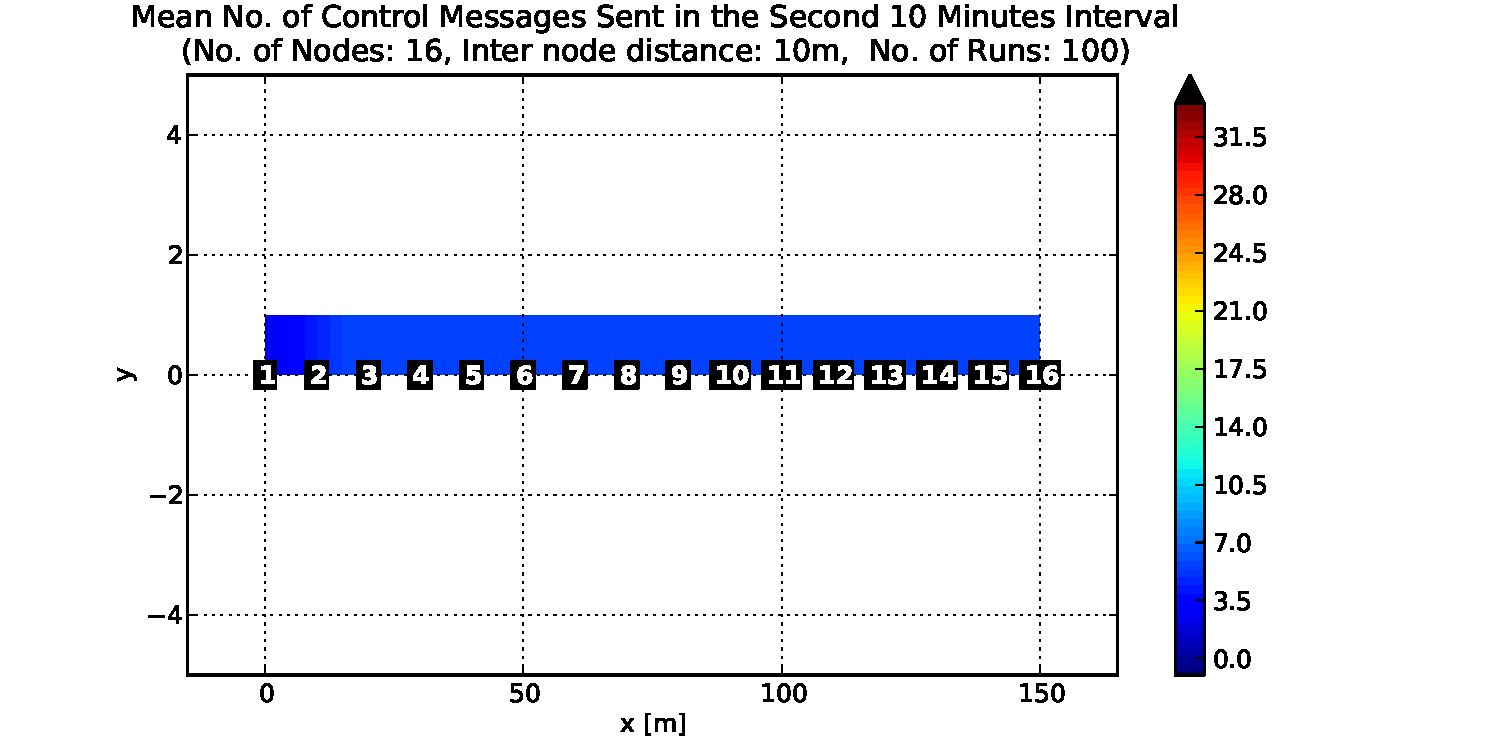
\includegraphics[trim=1.7cm 0cm 3cm 0cm, clip=true, scale=0.38]{Pics/results/16/MRHOF/line/dist10_montecarlo_contour_sent_ICMP_1.pdf}}
    \caption{Control message overhead: 16-node line scenario with 10 m internode distance}
    \label{fig:16_MRHOF_line_10_icmp}
  \end{center}
\end{figure}

\begin{figure}[htpb]
  \begin{center}
    \vspace{-10pt}
    \leavevmode
    \subfloat[First 10 minutes]{\label{fig:16_MRHOF_line_50_icmp0}
      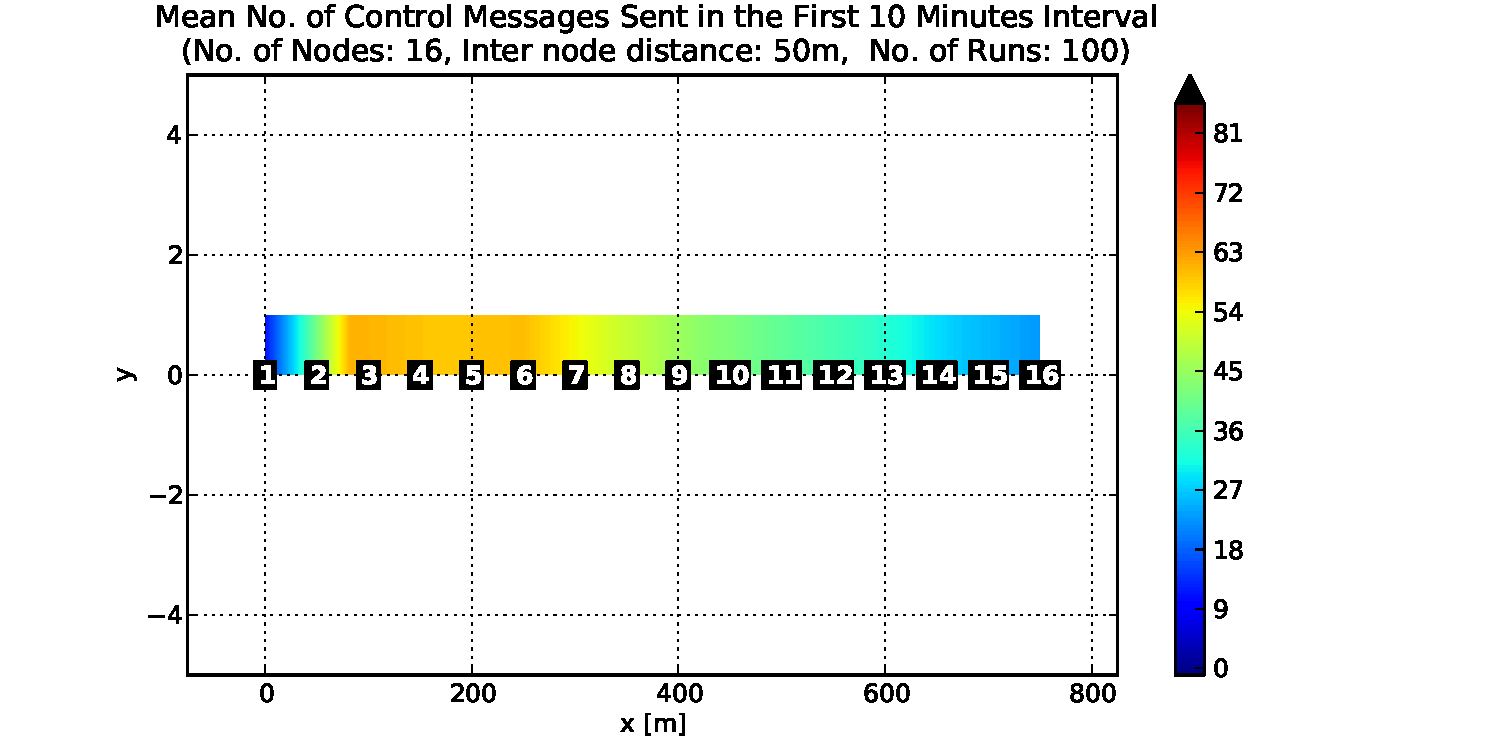
\includegraphics[trim=1.7cm 0cm 3cm 0cm, clip=true, scale=0.38]{Pics/results/16/MRHOF/line/dist50_montecarlo_contour_sent_ICMP_0.pdf}}
    \subfloat[Second 10 minutes]{\label{fig:16_MRHOF_line_50_icmp0}
       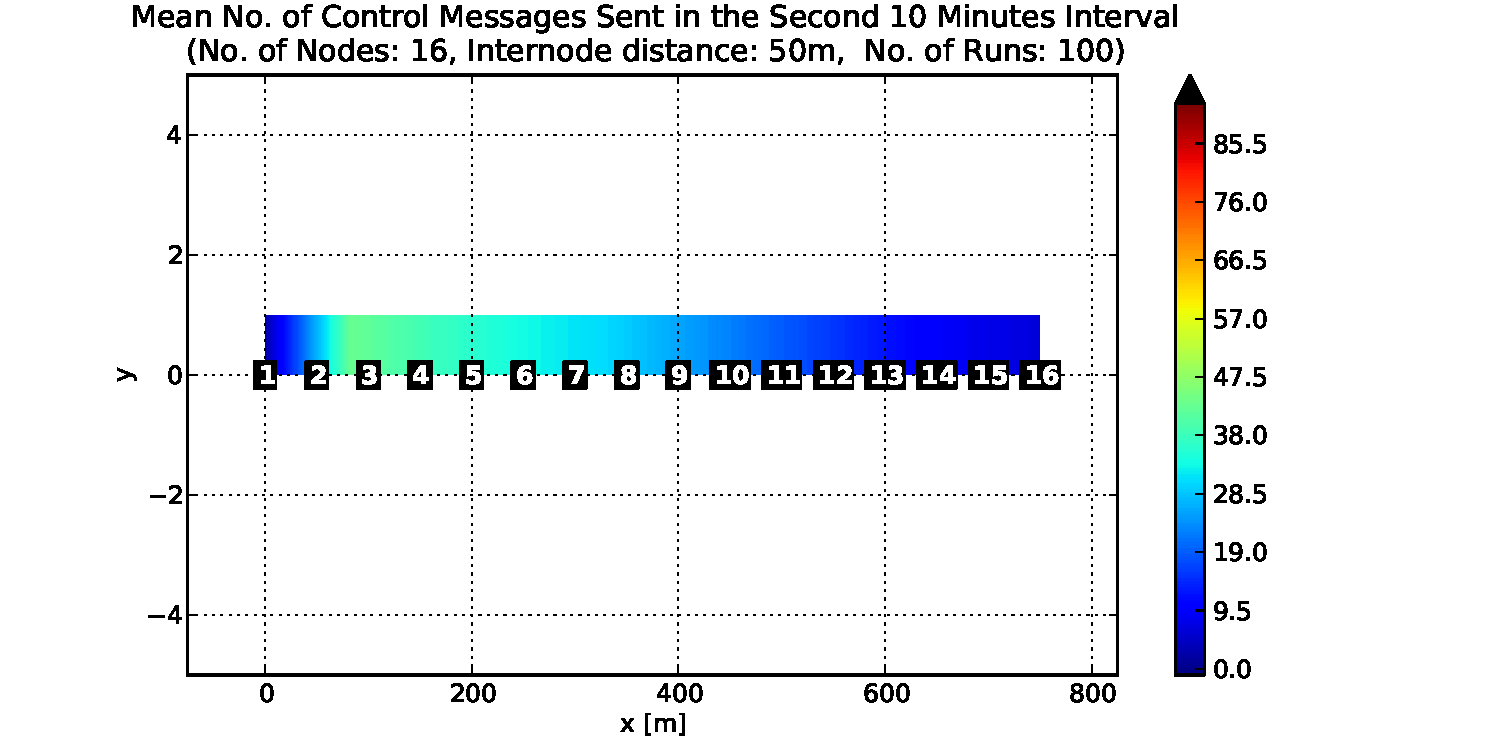
\includegraphics[trim=1.7cm 0cm 3cm 0cm, clip=true, scale=0.38]{Pics/results/16/MRHOF/line/dist50_montecarlo_contour_sent_ICMP_1.pdf}}
    \caption{Control message overhead: 16-node line scenario with 50 m internode distance}
    \label{fig:16_MRHOF_line_50_icmp}
  \end{center}
\end{figure}

\begin{figure}[htpb]
  \begin{center}
    \vspace{-10pt}
    \leavevmode
    \subfloat[First 10 minutes]{\label{fig:16_MRHOF_line_100_icmp0}
      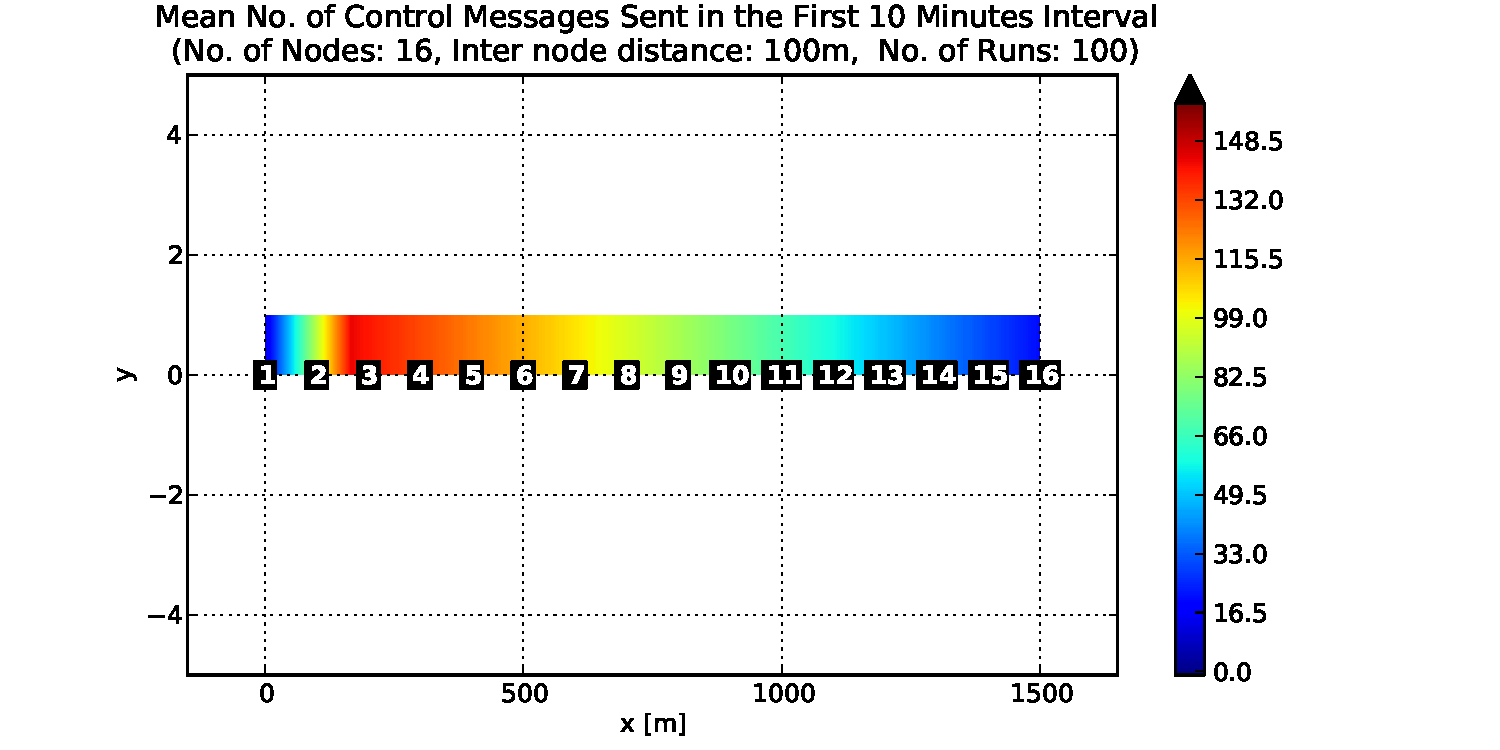
\includegraphics[trim=1.7cm 0cm 3cm 0cm, clip=true, scale=0.38]{Pics/results/16/MRHOF/line/dist100_montecarlo_contour_sent_ICMP_0}}
    \subfloat[Second 10 minutes]{\label{fig:16_MRHOF_line_100_icmp1}
       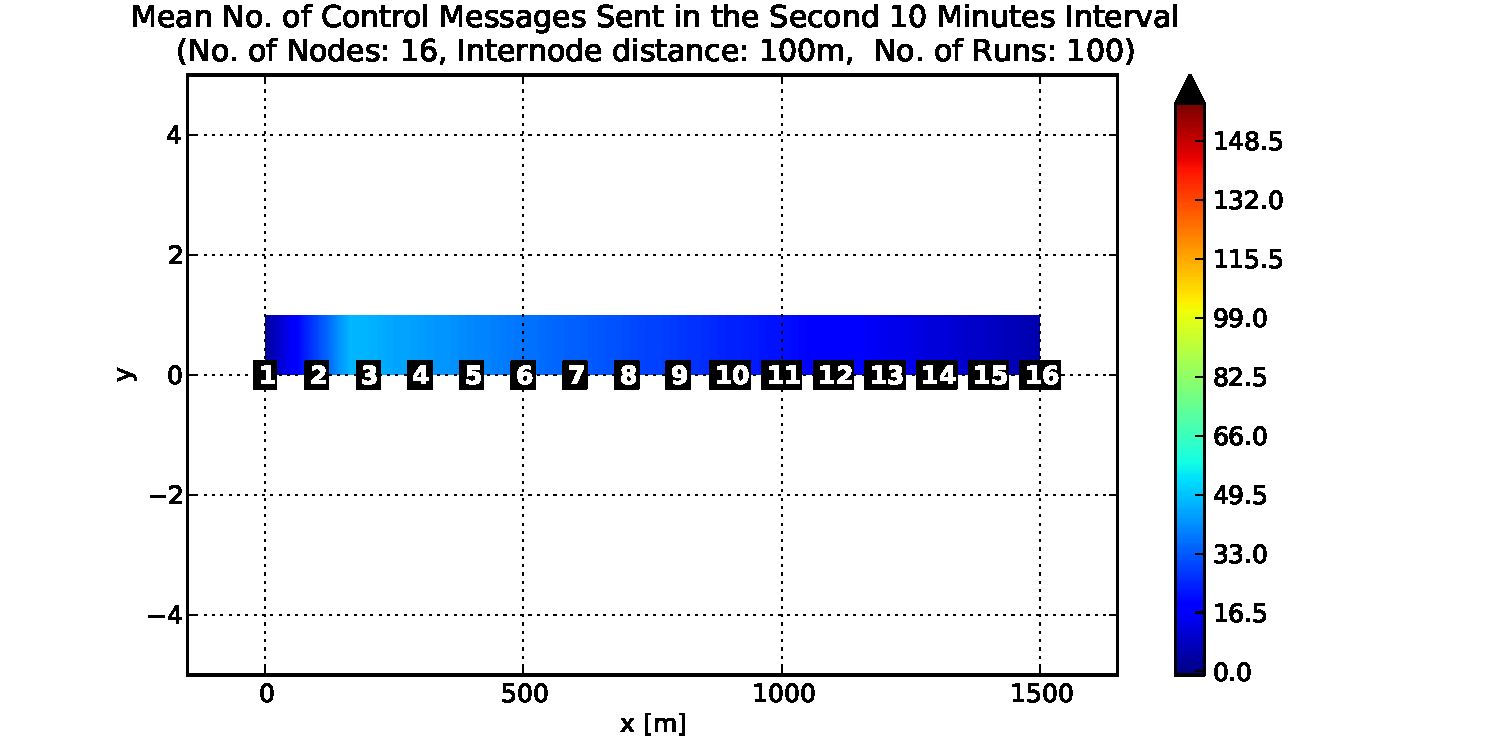
\includegraphics[trim=1.7cm 0cm 3cm 0cm, clip=true, scale=0.38]{Pics/results/16/MRHOF/line/dist100_montecarlo_contour_sent_ICMP_1}}
    \caption{Control message overhead: 16-node line scenario with 100 m internode distance}
    \label{fig:16_MRHOF_line_100_icmp}
  \end{center}
\end{figure}

\clearpage
\subsection{Grid Scenario}
\label{Appx:icmp:grid}
%%%%%%%%%%%%%%%%%%%%%%%%%%%%%%%%%%%%%%%%% grid 9 %%%%%%%%%%%%%%%%%%%%%%%%%%%%%%%%%%%%%%%%%%%%%%%%%%%%%%%%%%
\begin{figure}[htpb]
  \begin{center}
   \vspace{-20pt}
    \leavevmode
    \subfloat[First 10 minutes]{\label{fig:9_MRHOF_grid_10_icmp0}
      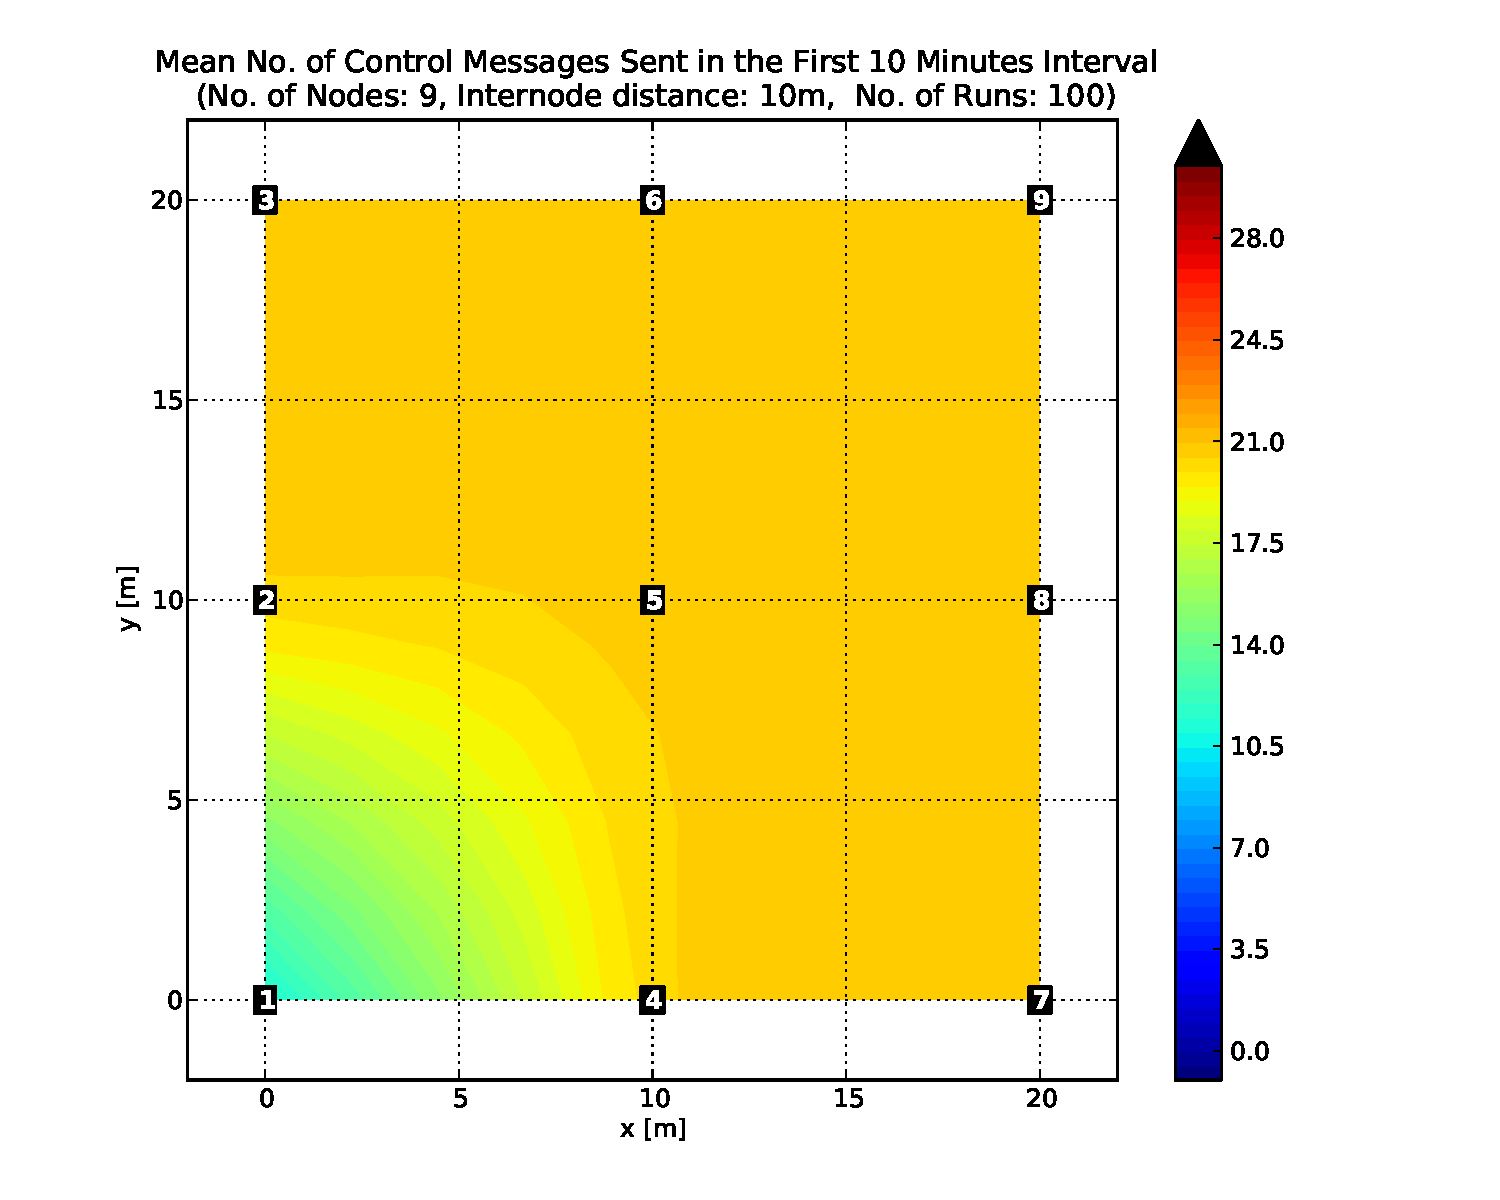
\includegraphics[trim=1cm 0cm 3cm 0cm, clip=true, scale=0.3]{Pics/results/9/MRHOF/grid/dist10_montecarlo_contour_sent_ICMP_0.pdf}}
    \subfloat[Second 10 minutes]{\label{fig:9_MRHOF_grid_10_icmp1}
       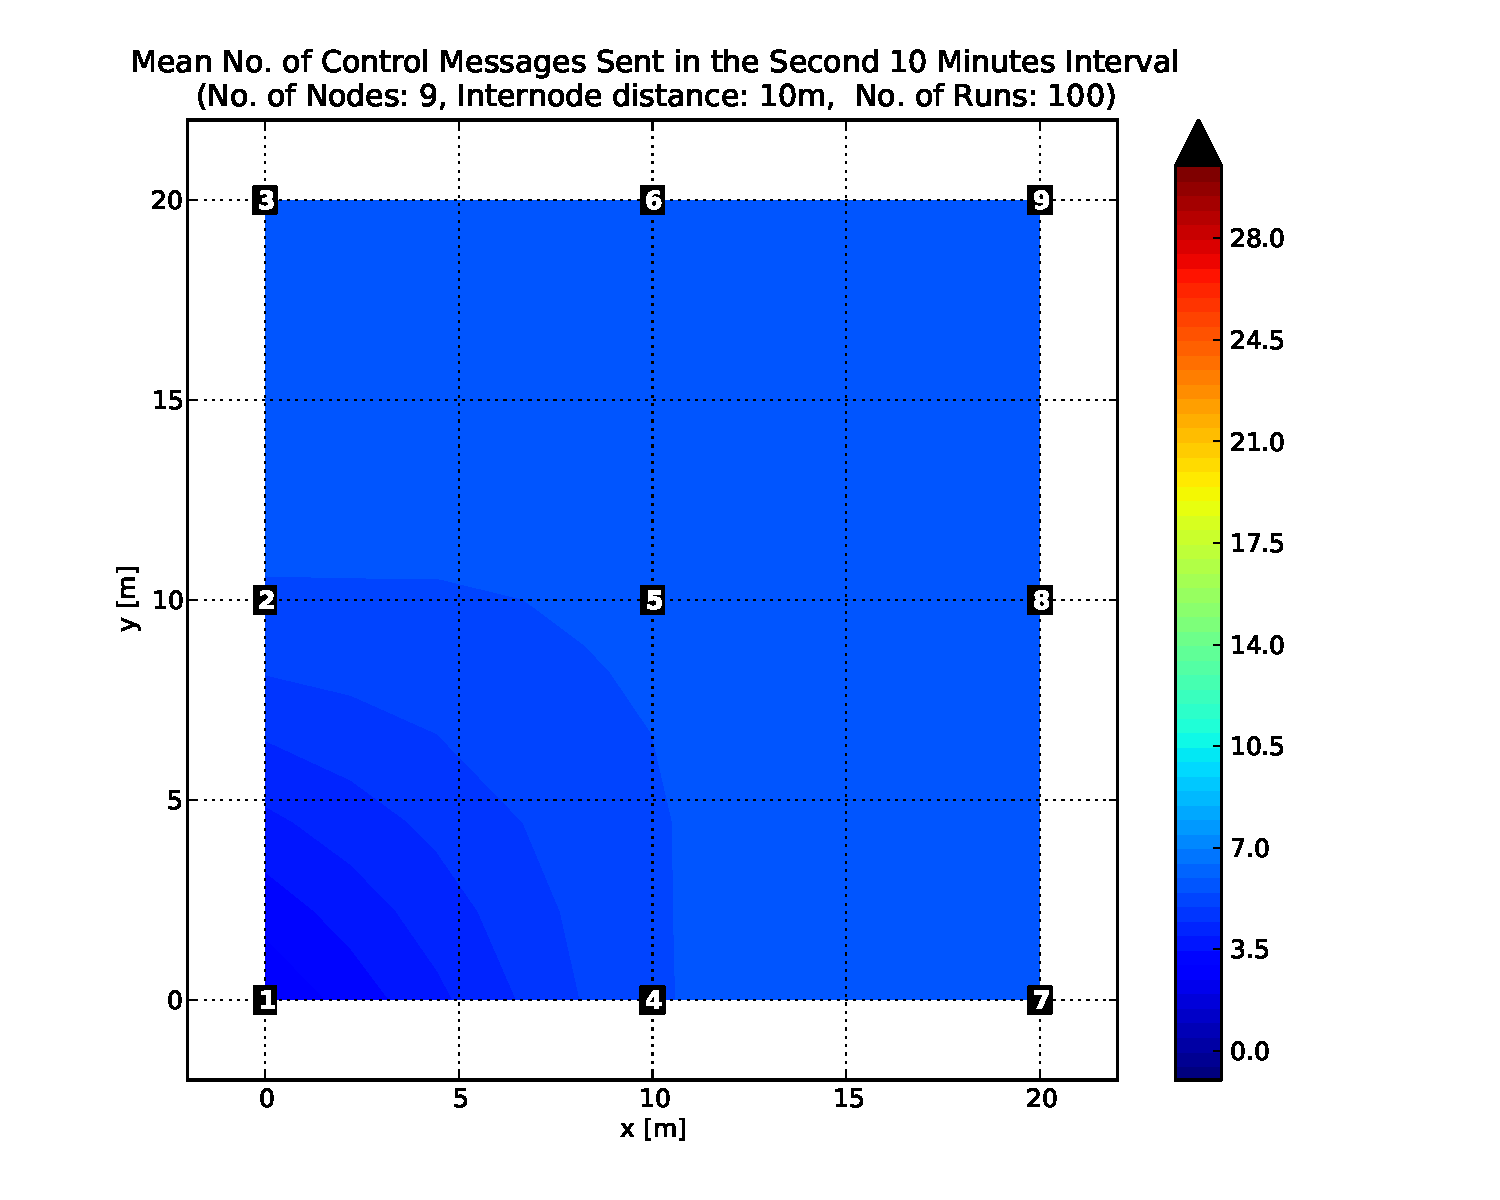
\includegraphics[trim=1cm 0cm 3cm 0cm, clip=true, scale=0.3]{Pics/results/9/MRHOF/grid/dist10_montecarlo_contour_sent_ICMP_1.pdf}}
    \caption{Control message overhead: 9-node grid scenario with 10 m internode distance}
    \label{fig:9_MRHOF_grid_10_icmp}
  \end{center}
   \vspace{-25pt}
\end{figure}

\begin{figure}[htpb]
  \begin{center}
    \leavevmode
    \subfloat[First 10 minutes]{\label{fig:9_MRHOF_grid_50_icmp0}
      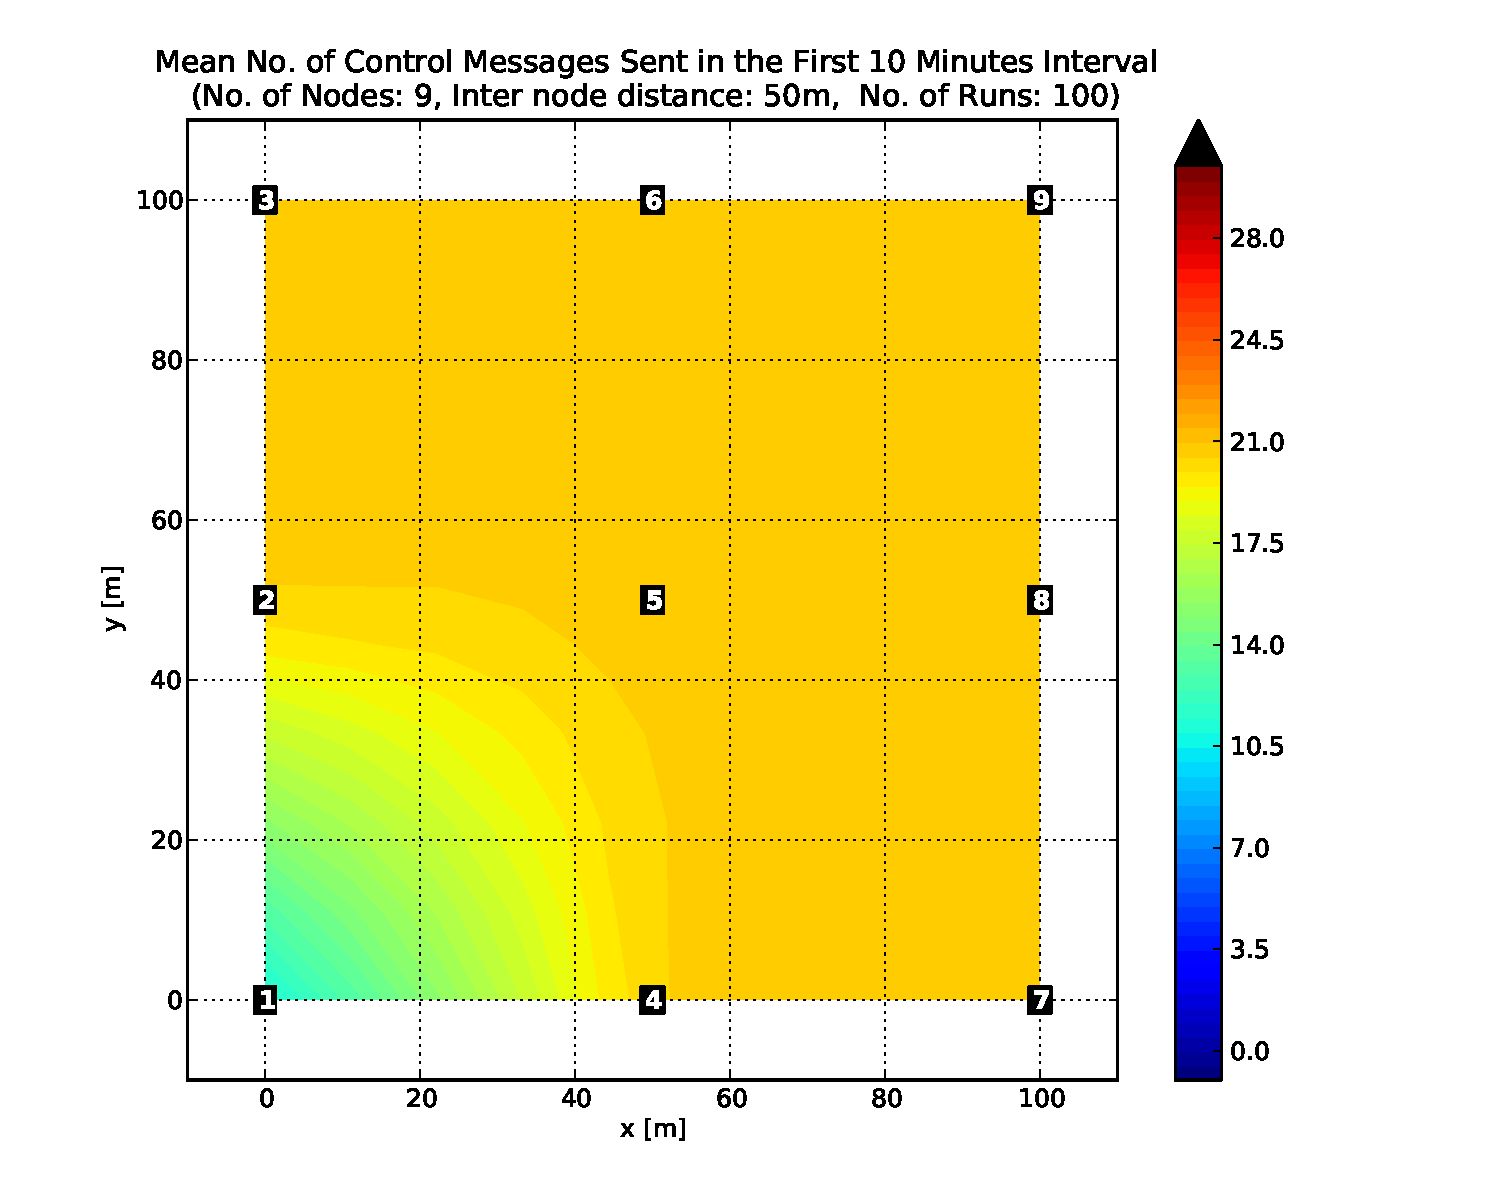
\includegraphics[trim=1cm 0cm 3cm 0cm, clip=true, scale=0.3]{Pics/results/9/MRHOF/grid/dist50_montecarlo_contour_sent_ICMP_0.pdf}}
    \subfloat[Second 10 minutes]{\label{fig:9_MRHOF_grid_50_icmp0}
       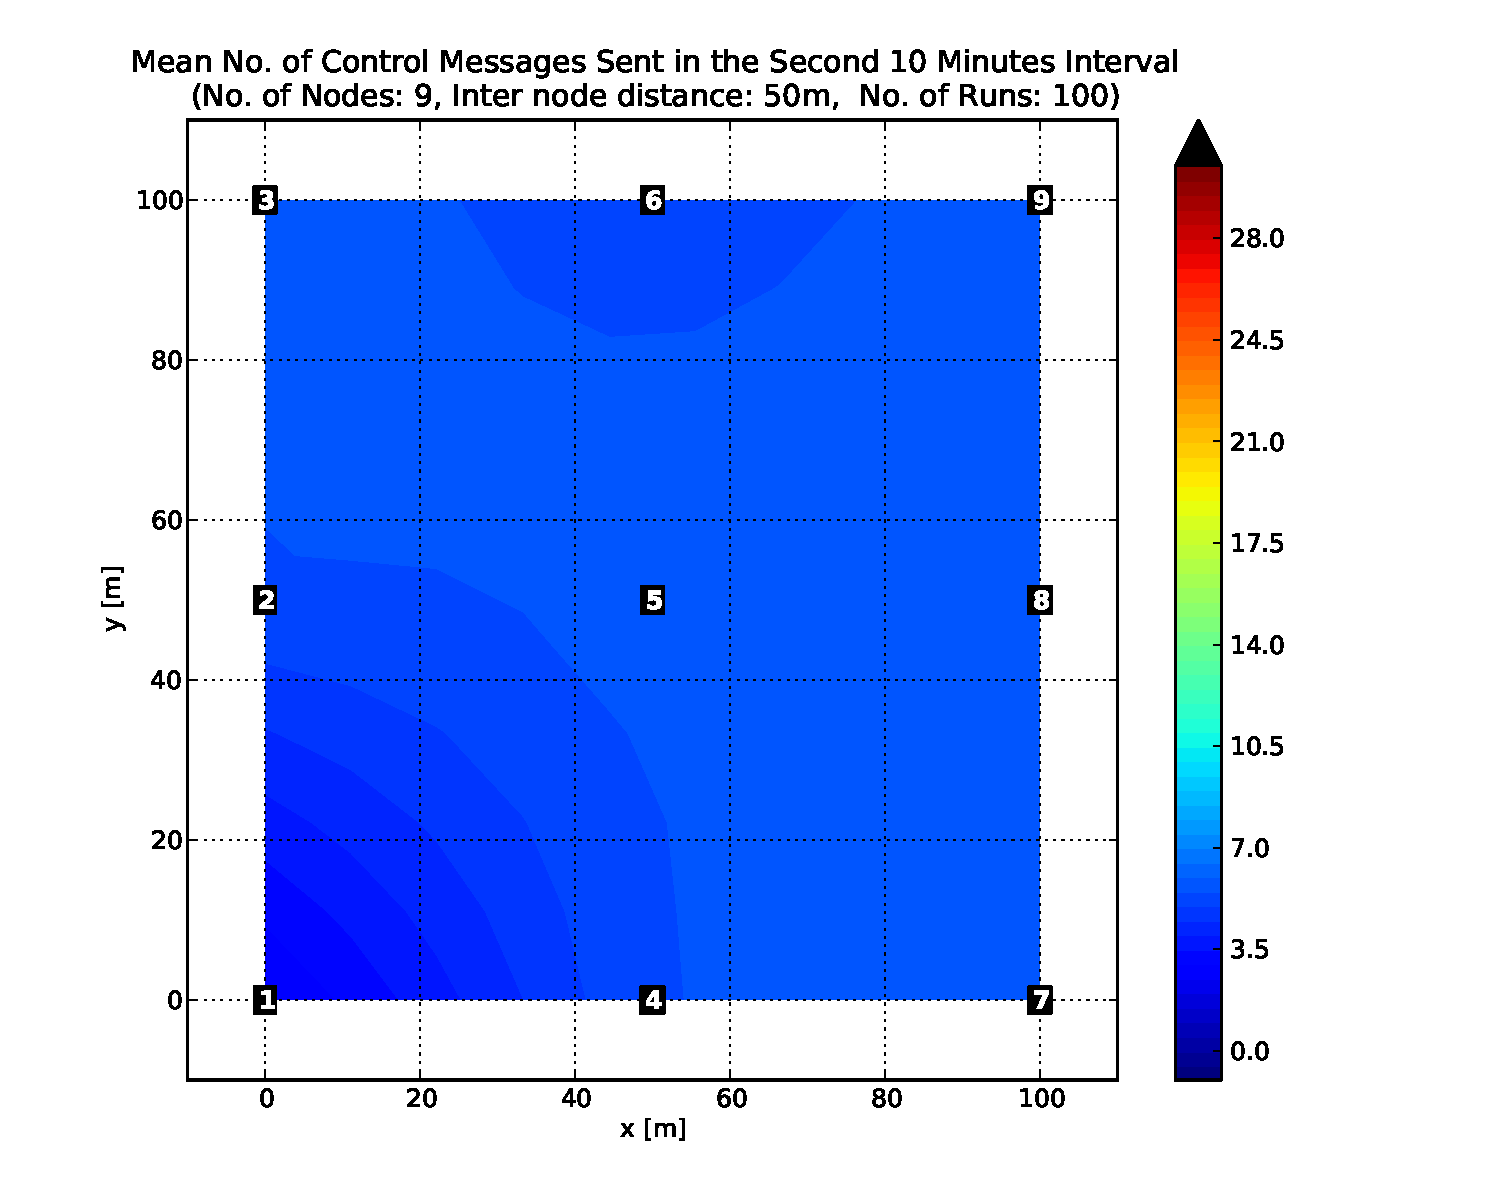
\includegraphics[trim=1cm 0cm 3cm 0cm, clip=true, scale=0.3]{Pics/results/9/MRHOF/grid/dist50_montecarlo_contour_sent_ICMP_1.pdf}}
    \caption{Control message overhead: 9-node grid scenario with 50 m internode distance}
    \label{fig:9_MRHOF_grid_50_icmp}
  \end{center}
   \vspace{-25pt}
\end{figure}

\begin{figure}[htpb]
  \begin{center}
    \leavevmode
    \subfloat[First 10 minutes]{\label{fig:9_MRHOF_grid_100_icmp0}
      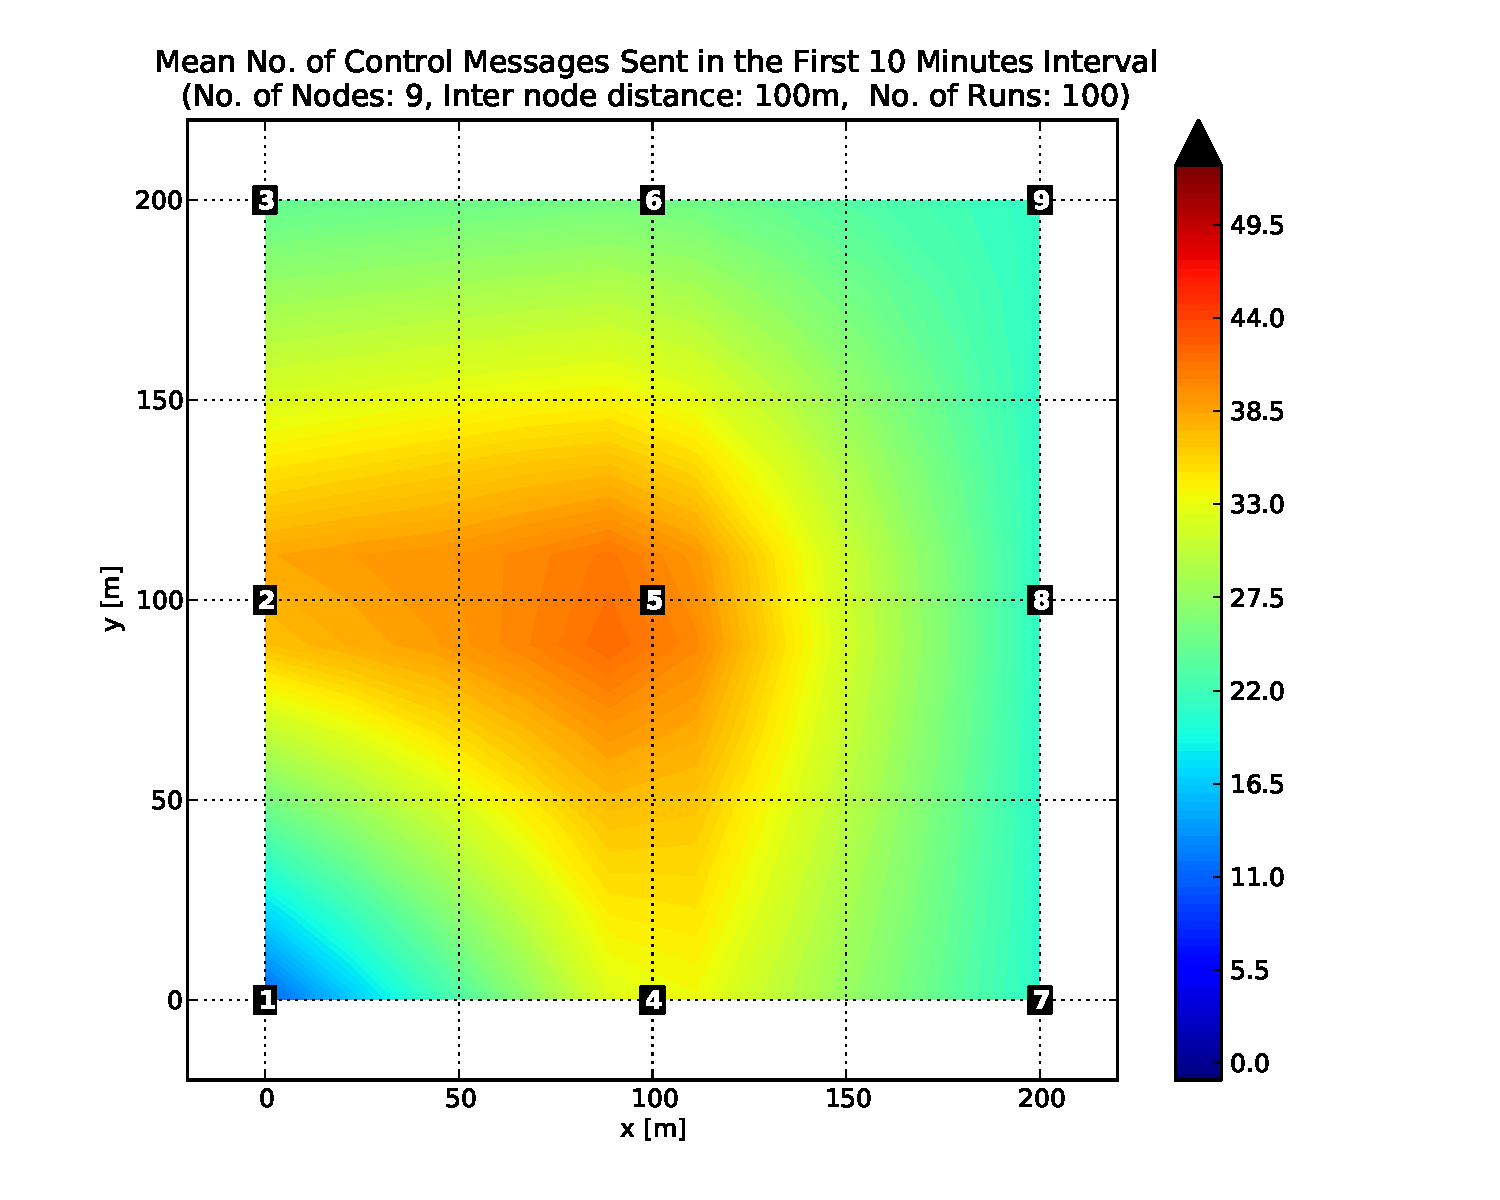
\includegraphics[trim=1cm 0cm 3cm 0cm, clip=true, scale=0.3]{Pics/results/9/MRHOF/grid/dist100_montecarlo_contour_sent_ICMP_0}}
    \subfloat[Second 10 minutes]{\label{fig:9_MRHOF_grid_100_icmp1}
       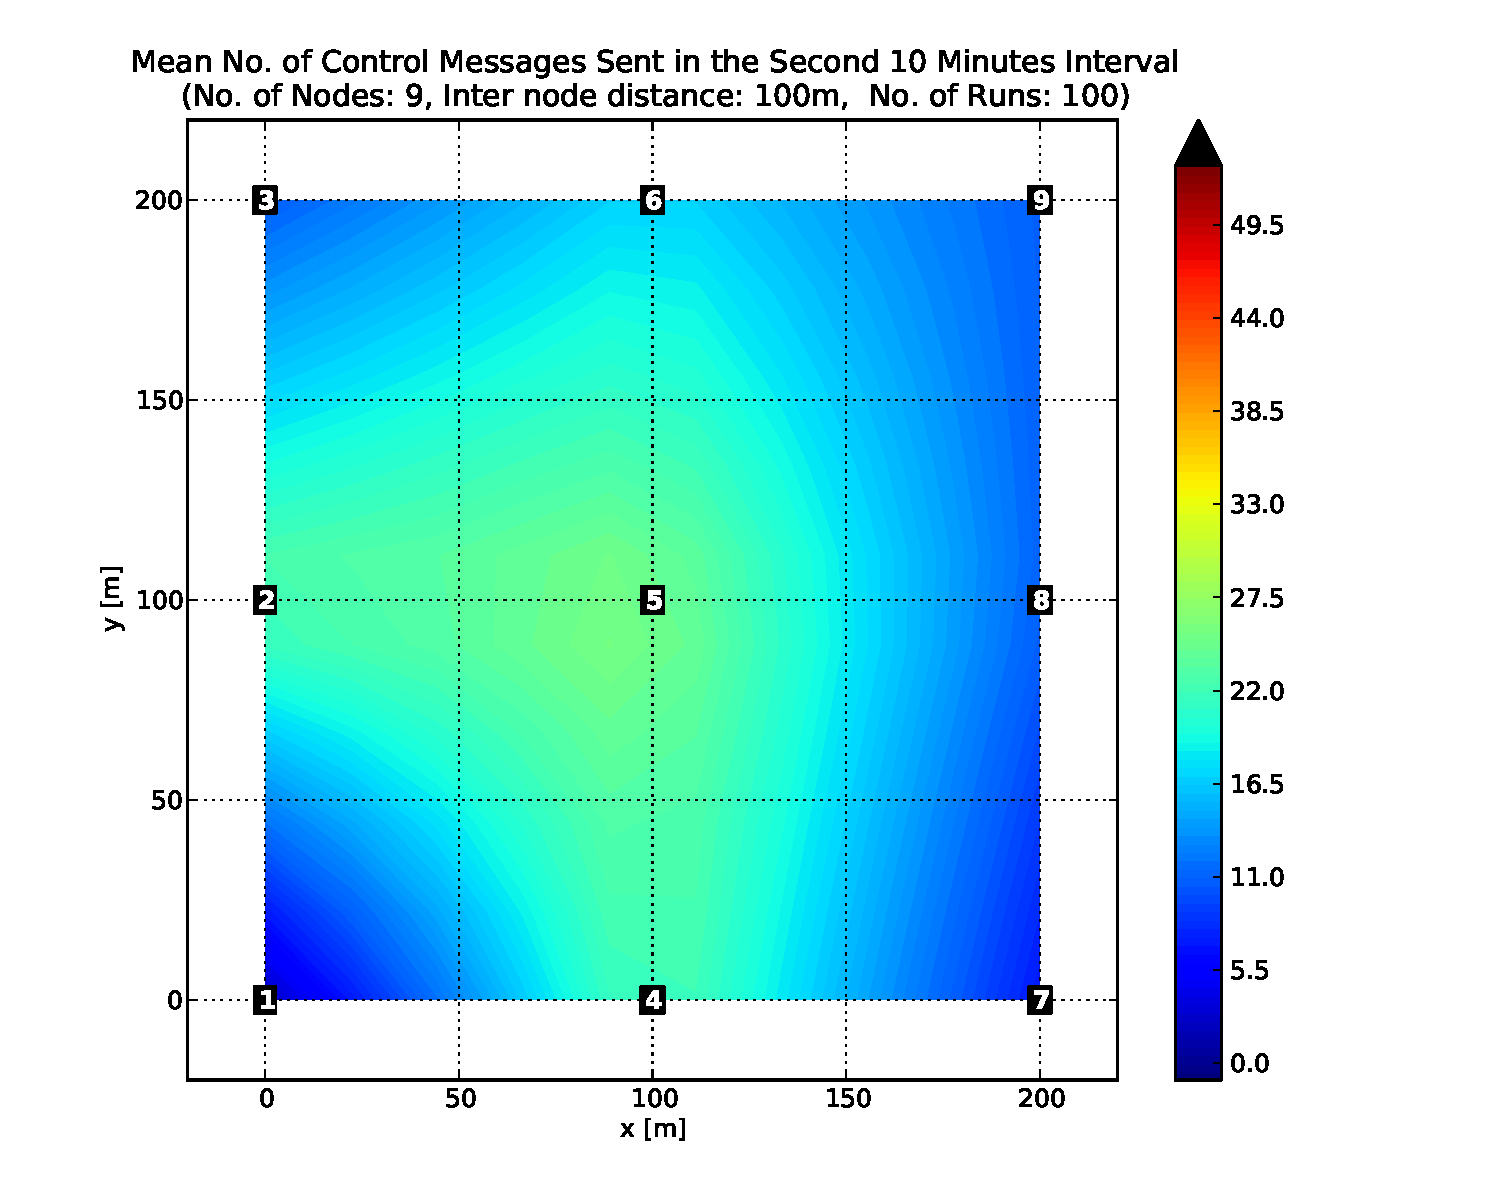
\includegraphics[trim=1cm 0cm 3cm 0cm, clip=true, scale=0.3]{Pics/results/9/MRHOF/grid/dist100_montecarlo_contour_sent_ICMP_1}}
    \caption{Control message overhead: 9-node grid scenario with 100 m internode distance}
    \label{fig:9_MRHOF_grid_100_icmp}
  \end{center}
   \vspace{-25pt}
\end{figure}

%%%%%%%%%%%%%%%%%%%%%%%%%%%%%%%%%%%%%% grid 16 %%%%%%%%%%%%%%%%%%%%%%%%%%%%%%%%%%%%%%%%%%%%%%%%%
\begin{figure}[htpb]
  \begin{center}
   \vspace{-20pt}
    \leavevmode
    \subfloat[First 10 minutes]{\label{fig:16_MRHOF_grid_10_icmp0}
      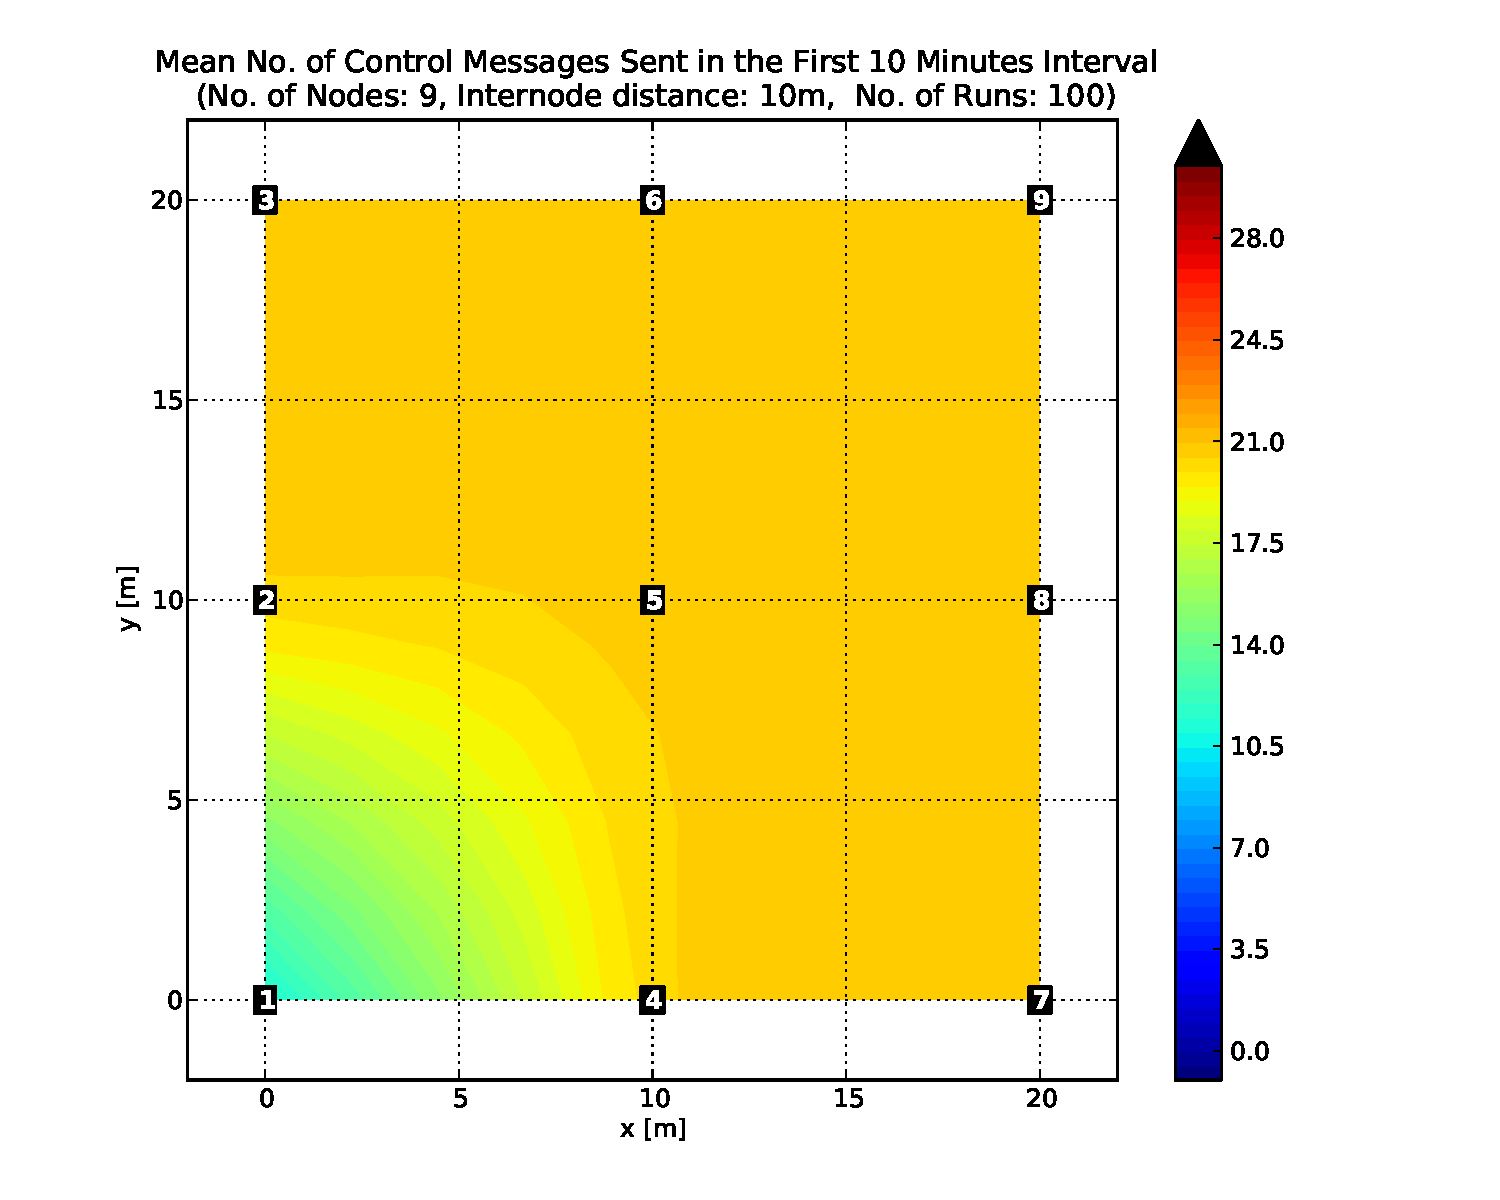
\includegraphics[trim=1cm 0cm 3cm 0cm, clip=true, scale=0.32]{Pics/results/9/MRHOF/grid/dist10_montecarlo_contour_sent_ICMP_0.pdf}}
    \subfloat[Second 10 minutes]{\label{fig:16_MRHOF_grid_10_icmp1}
       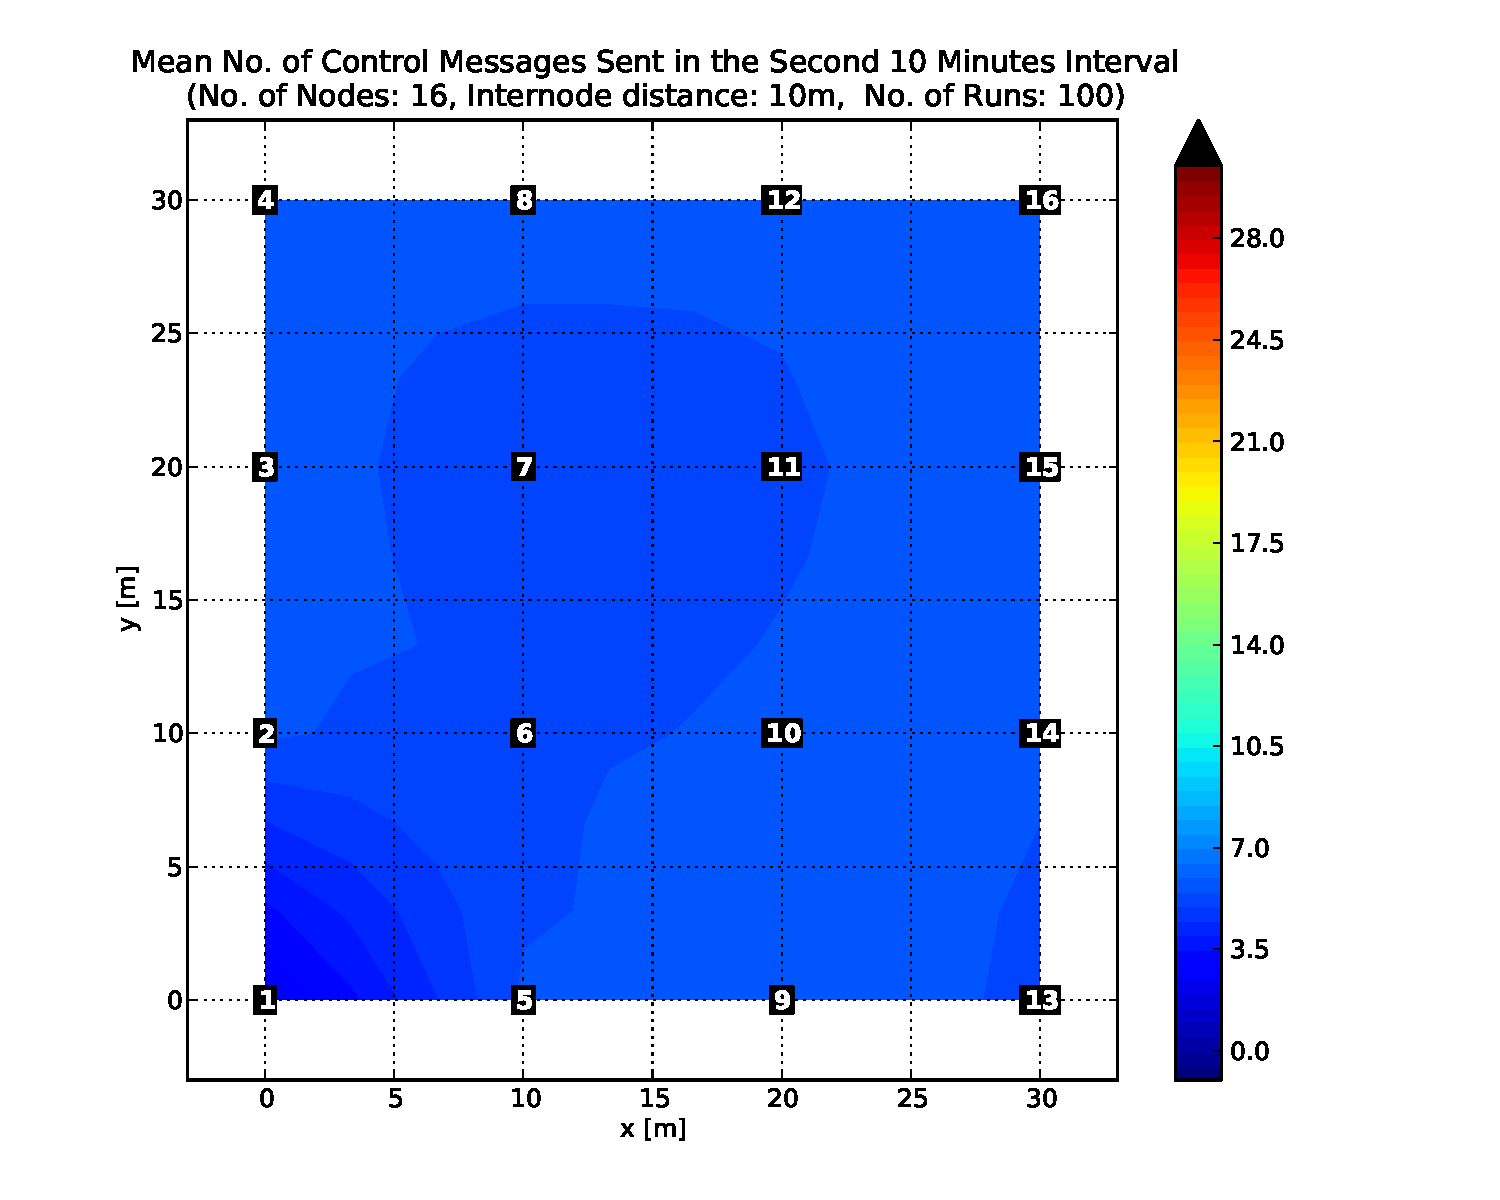
\includegraphics[trim=1cm 0cm 3cm 0cm, clip=true, scale=0.32]{Pics/results/16/MRHOF/grid/dist10_montecarlo_contour_sent_ICMP_1.pdf}}
    \caption{Control message overhead: 16-node grid scenario with 10 m internode distance}
    \label{fig:16_MRHOF_grid_10_icmp}
  \end{center}
   \vspace{-25pt}
\end{figure}

\begin{figure}[htpb]
  \begin{center}
    \leavevmode
    \subfloat[First 10 minutes]{\label{fig:16_MRHOF_grid_50_icmp0}
      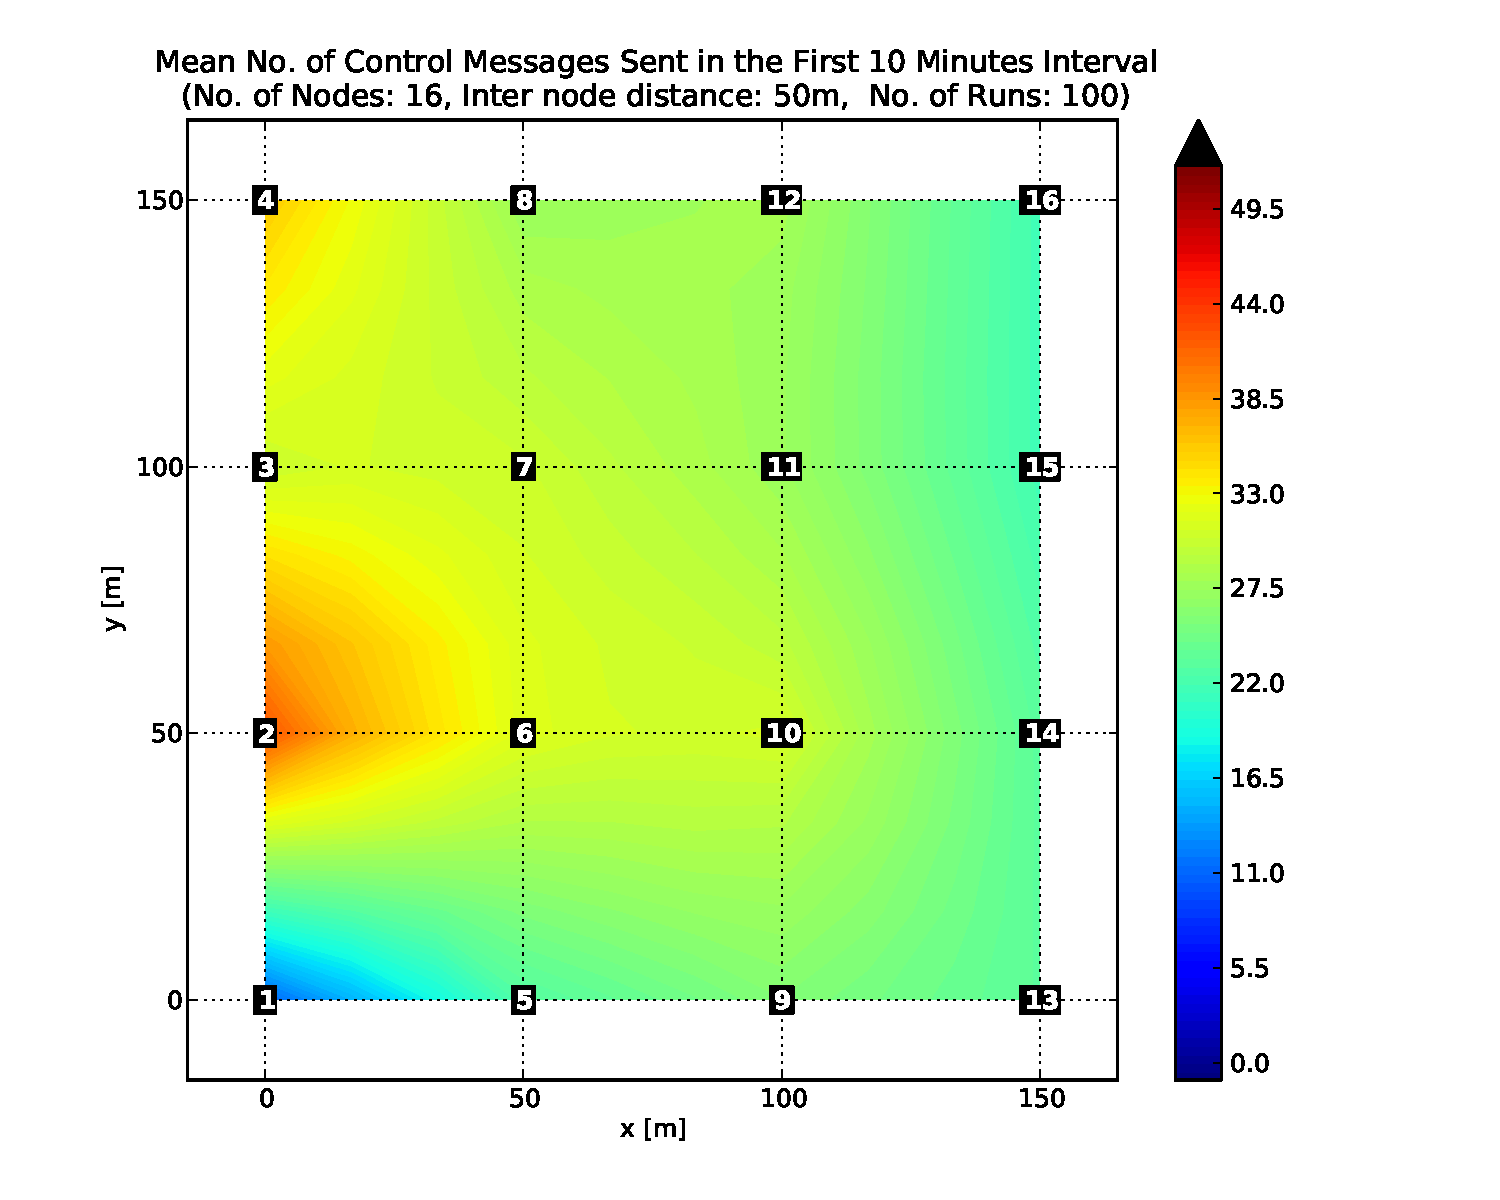
\includegraphics[trim=1cm 0cm 3cm 0cm, clip=true, scale=0.32]{Pics/results/16/MRHOF/grid/dist50_montecarlo_contour_sent_ICMP_0.pdf}}
    \subfloat[Second 10 minutes]{\label{fig:16_MRHOF_grid_50_icmp0}
       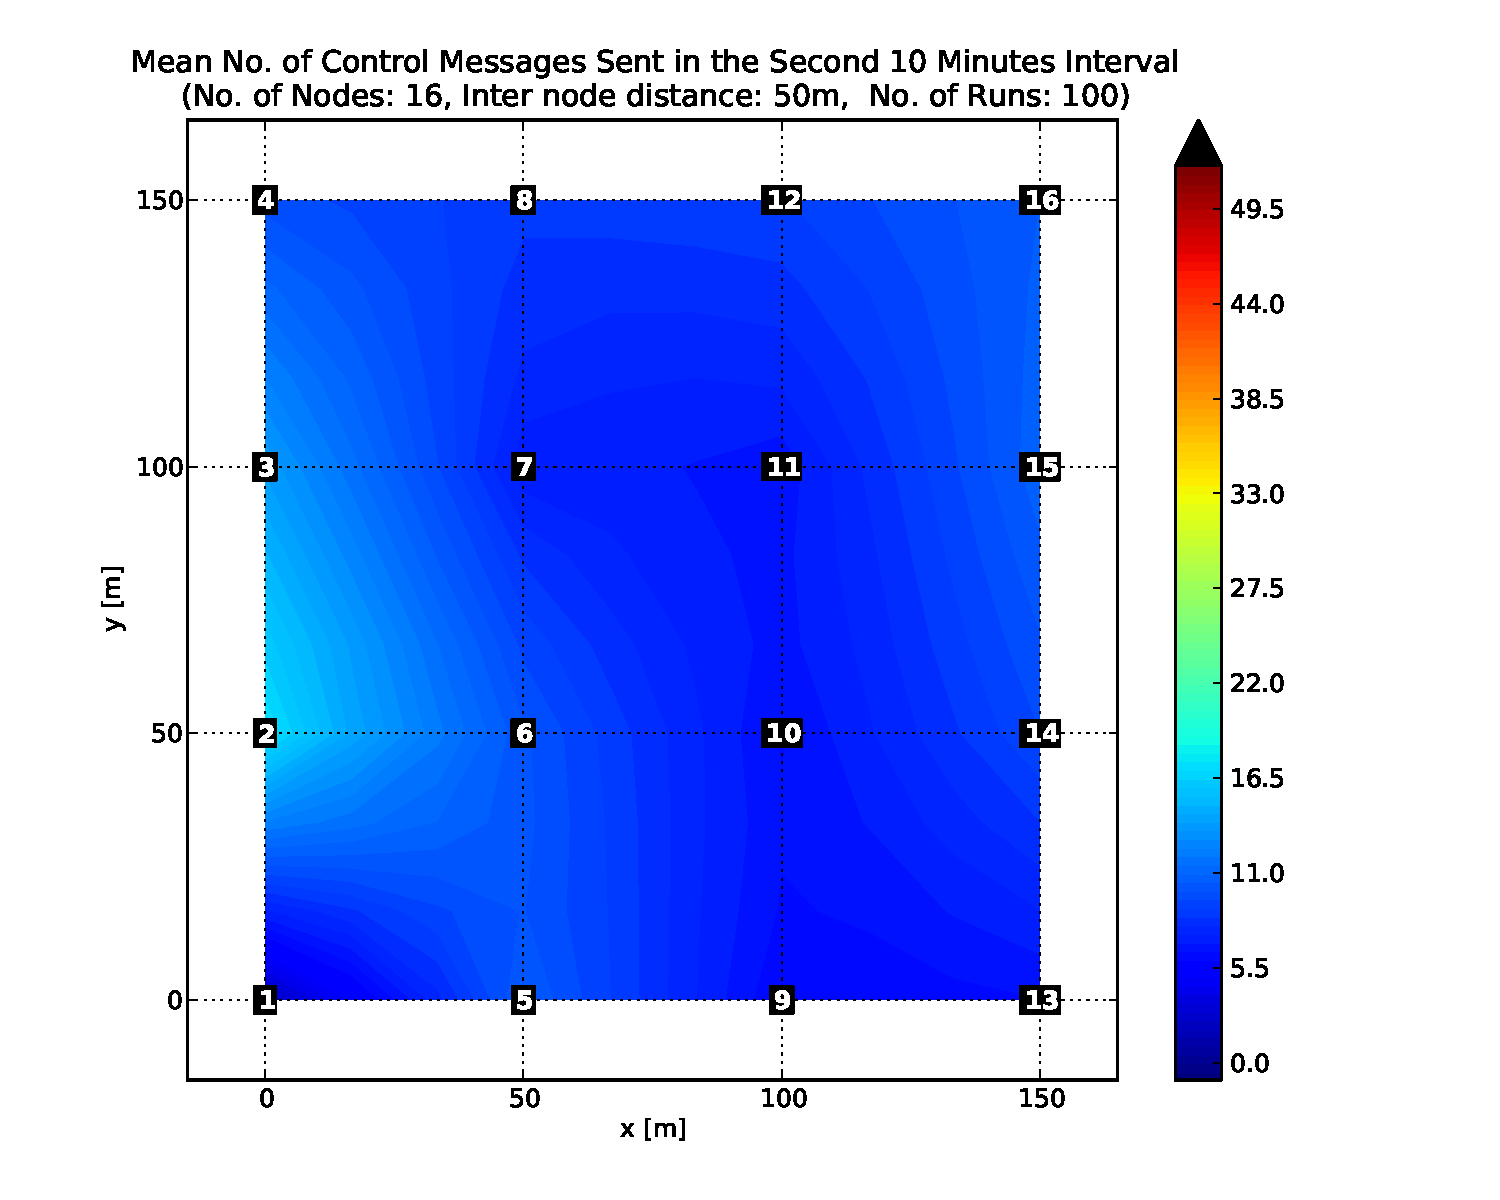
\includegraphics[trim=1cm 0cm 3cm 0cm, clip=true, scale=0.32]{Pics/results/16/MRHOF/grid/dist50_montecarlo_contour_sent_ICMP_1.pdf}}
    \caption{Control message overhead: 16-node grid scenario with 50 m internode distance}
    \label{fig:16_MRHOF_grid_50_icmp}
  \end{center}
   \vspace{-25pt}
\end{figure}

\begin{figure}[htpb]
  \begin{center}
    \leavevmode
    \subfloat[First 10 minutes]{\label{fig:16_MRHOF_grid_100_icmp0}
      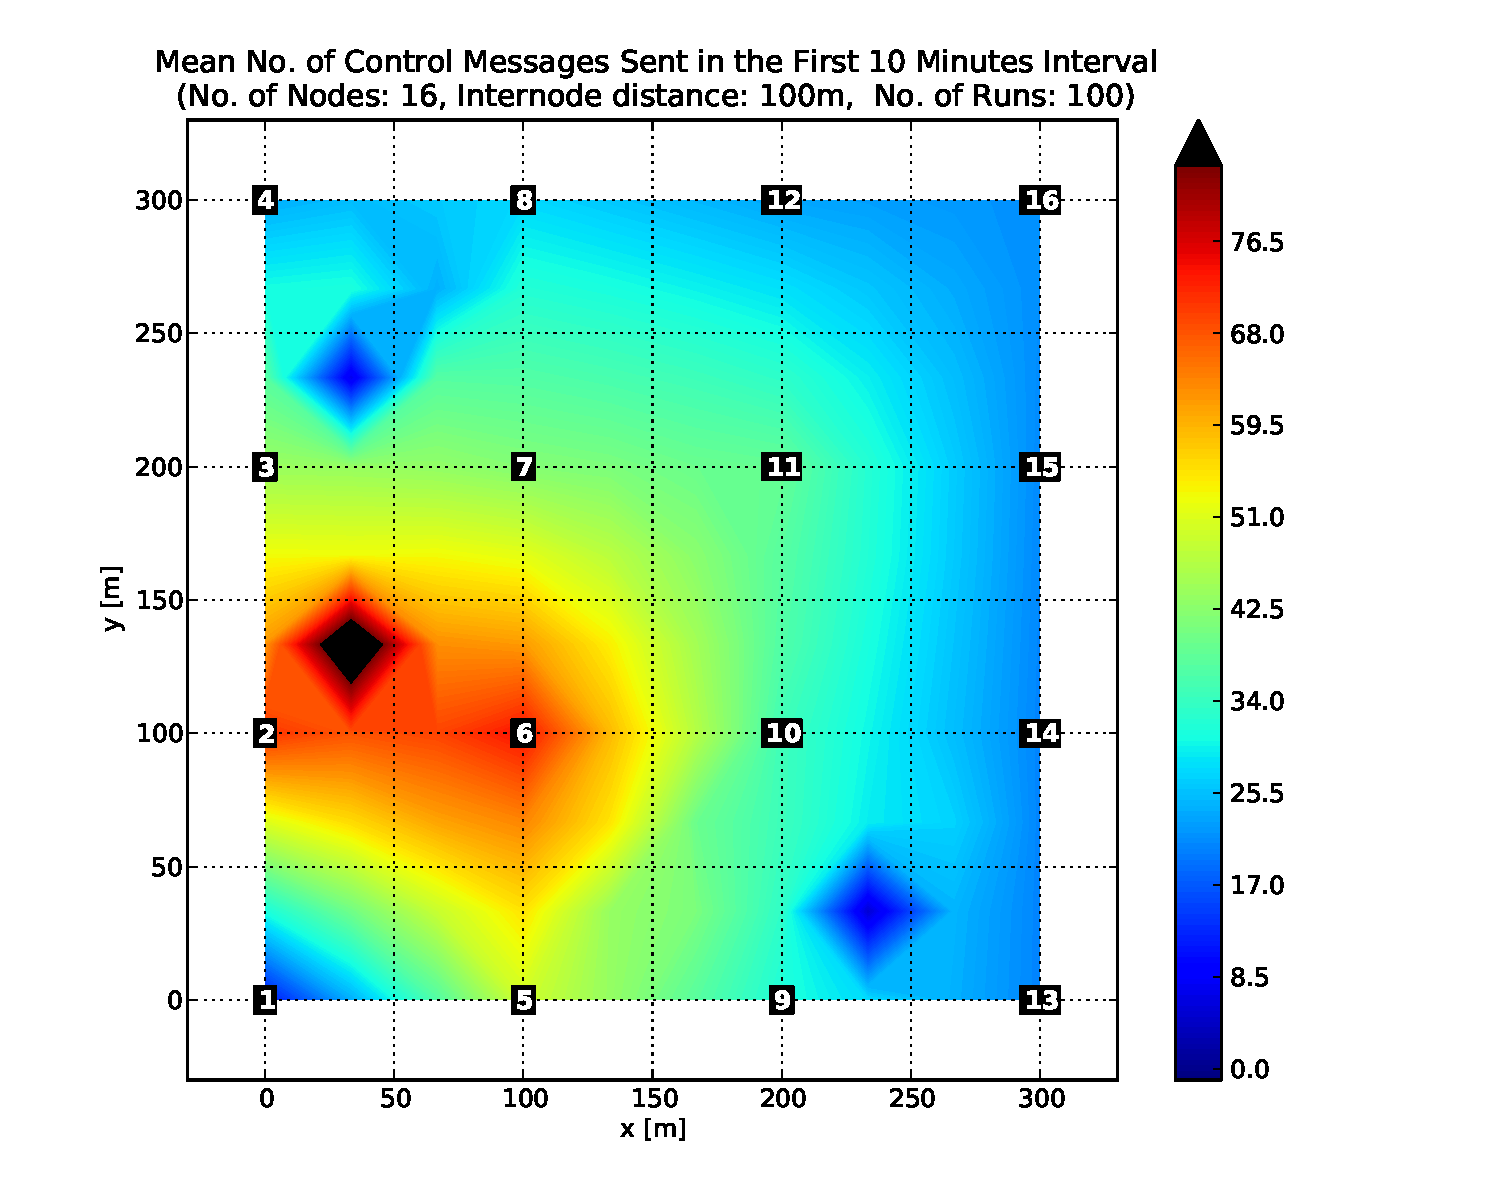
\includegraphics[trim=1cm 0cm 3cm 0cm, clip=true, scale=0.32]{Pics/results/16/MRHOF/grid/dist100_montecarlo_contour_sent_ICMP_0}}
    \subfloat[Second 10 minutes]{\label{fig:16_MRHOF_grid_100_icmp1}
       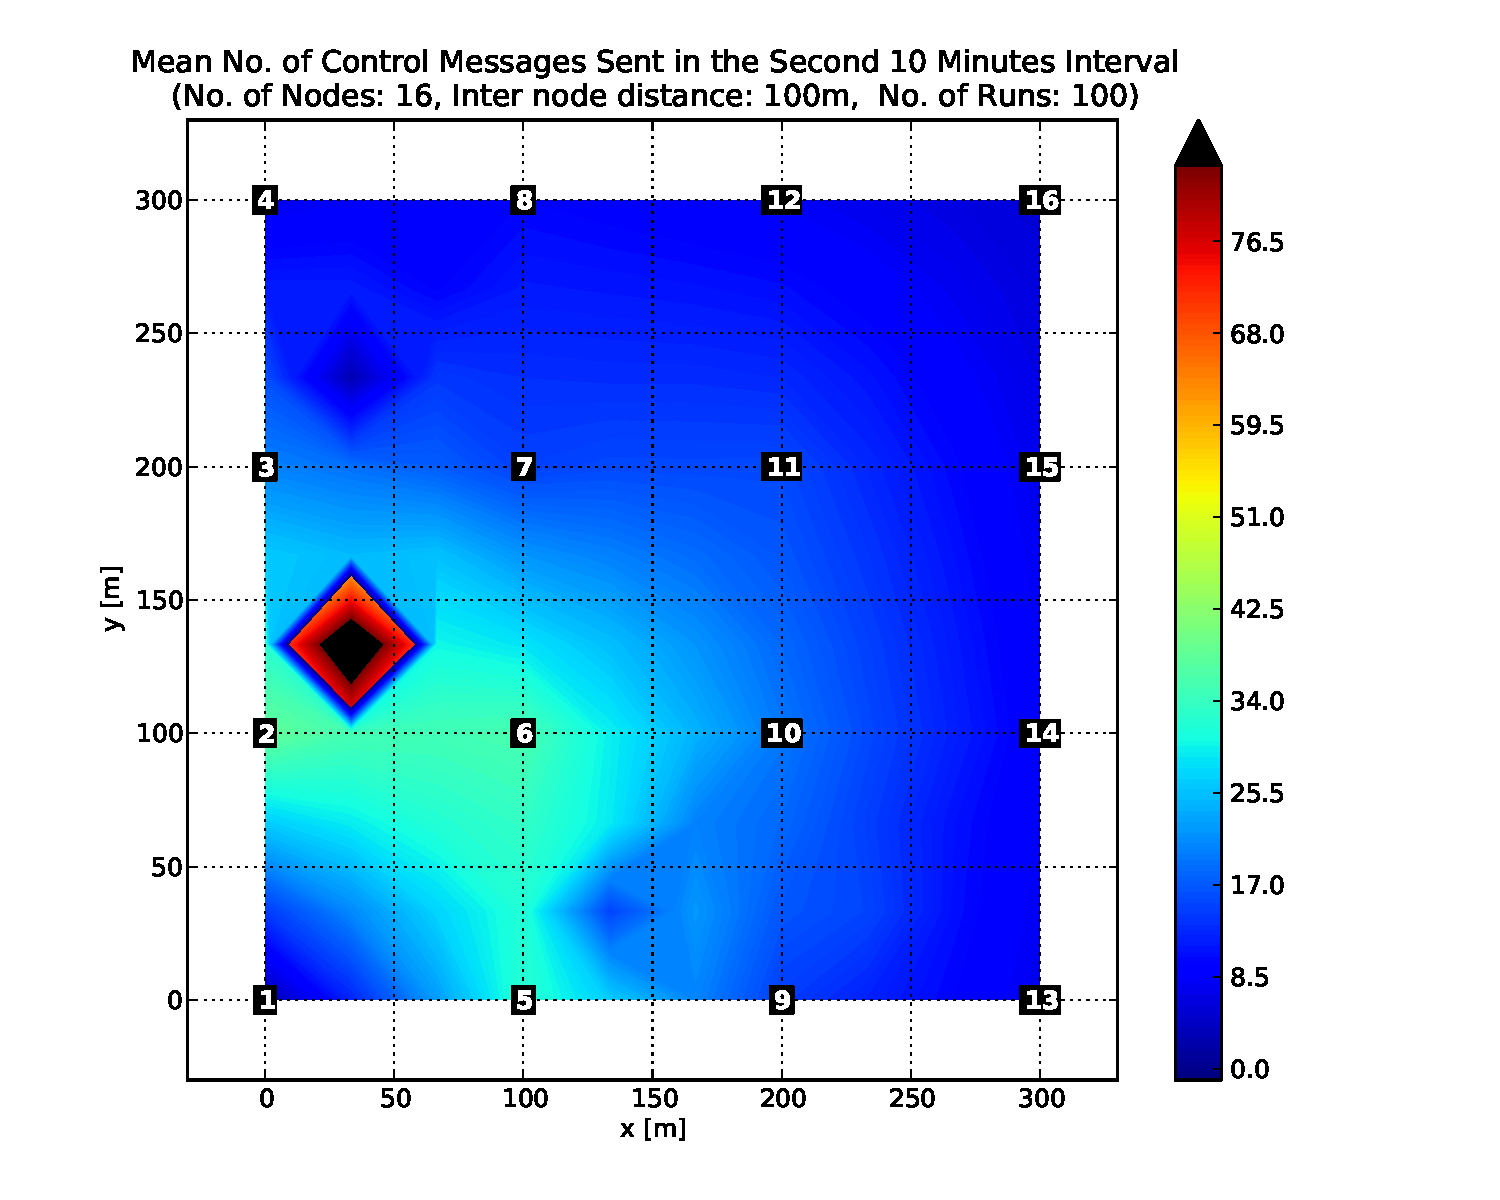
\includegraphics[trim=1cm 0cm 3cm 0cm, clip=true, scale=0.32]{Pics/results/16/MRHOF/grid/dist100_montecarlo_contour_sent_ICMP_1}}
    \caption{Control message overhead: 16-node grid scenario with 100 m internode distance}
    \label{fig:16_MRHOF_grid_100_icmp}
  \end{center}
  \vspace{-25pt}
\end{figure}